% !TeX program = xelatex
% !TeX encoding = UTF-8
\RequirePackage{fix-cm}
\documentclass[12pt,a4paper,oneside]{report}

\usepackage{iftex}
\ifPDFTeX
  \errmessage{Hay bien dich bang XeLaTeX, LuaLaTeX hoac Tectonic de hien thi tieng Viet}
\fi
\usepackage{fontspec}
\IfFontExistsTF{Times New Roman}
  {\setmainfont{Times New Roman}}
  {\setmainfont{TeX Gyre Termes}}
\IfFontExistsTF{Arial}
  {\setsansfont{Arial}}
  {\setsansfont{TeX Gyre Heros}}
\IfFontExistsTF{Courier New}
  {\setmonofont{Courier New}[Scale=MatchLowercase]}
  {\setmonofont{lmmono10-regular.otf}[Scale=MatchLowercase]}
\usepackage[vietnamese]{babel}
\usepackage[left=3cm,right=2cm,top=2.5cm,bottom=2.5cm,headheight=17pt]{geometry}
\usepackage{amsmath,amssymb}
\usepackage{graphicx}
\usepackage{listings}
\lstset{
  language=Python,
  basicstyle=\ttfamily\footnotesize,
  keywordstyle=\bfseries,
  commentstyle=\itshape,
  frame=single,
  framerule=0.3pt,
  aboveskip=8pt,
  belowskip=8pt,
  xleftmargin=4pt,
  xrightmargin=4pt,
  breaklines=true,
  breakatwhitespace=false,
  columns=fullflexible,
  keepspaces=true,
  showstringspaces=false,
  tabsize=4,
  upquote=true
}
\usepackage{booktabs,tabularx,array}
\usepackage{enumitem}
\usepackage{setspace}
\usepackage{titlesec}
\usepackage{fancyhdr}
\usepackage{caption}
\PassOptionsToPackage{obeyspaces}{url}
\usepackage{xurl}
\usepackage[hidelinks,unicode]{hyperref}

% report hỗ trợ tùy chọn 12 pt; đặt cỡ thân bài 13 pt một cách tường minh.
\makeatletter
\renewcommand\normalsize{%
  \@setfontsize\normalsize{13pt}{16pt}%
  \abovedisplayskip 10pt plus 2pt minus 5pt
  \abovedisplayshortskip 0pt plus 3pt
  \belowdisplayshortskip 6pt plus 3pt minus 3pt
  \belowdisplayskip \abovedisplayskip
  \let\@listi\@listI}
\makeatother
\normalsize
\DeclareMathSizes{13}{13}{9}{7}
\setstretch{1.25}
\widowpenalty=10000
\clubpenalty=10000
\displaywidowpenalty=10000
\setlength{\parindent}{1cm}
\setlength{\parskip}{3pt}
\setlength{\emergencystretch}{2em}
\setlist[itemize]{leftmargin=1.5em,itemsep=2pt,topsep=4pt}
\setlist[enumerate]{leftmargin=1.8em,itemsep=2pt,topsep=4pt}
\setcounter{tocdepth}{2}
\setcounter{secnumdepth}{2}
\renewcommand{\arraystretch}{1.15}
\newcolumntype{Y}{>{\raggedright\arraybackslash}X}
\captionsetup{font=small,labelfont=bf,labelsep=period}
\titleformat{\chapter}[display]
  {\normalfont\bfseries\centering\Large}
  {CHƯƠNG \thechapter}{0.5em}{}
\titlespacing*{\chapter}{0pt}{0pt}{1.5em}
\titleformat{\section}{\normalfont\bfseries\large}{\thesection}{0.7em}{}
\titleformat{\subsection}{\normalfont\bfseries}{\thesubsection}{0.7em}{}
\titlespacing*{\section}{0pt}{1.2em}{0.5em}
\titlespacing*{\subsection}{0pt}{0.8em}{0.3em}
\pagestyle{fancy}
\fancyhf{}
\fancyhead[L]{\small\itshape Tiểu luận môn Trực quan hóa dữ liệu}
\fancyfoot[C]{\thepage}
\renewcommand{\headrulewidth}{0.3pt}
\urlstyle{same}
\fancypagestyle{plain}{%
  \fancyhf{}\fancyfoot[C]{\thepage}\renewcommand{\headrulewidth}{0pt}}
\hypersetup{
  pdftitle={Trực quan hóa và phân tích dữ liệu lỗi bề mặt thép bằng Python},
  pdfsubject={Tiểu luận: Phần mở đầu và các Chương 1, 2, 3, 4},
  pdfkeywords={trực quan hóa dữ liệu, lỗi bề mặt thép, Python, dashboard}
}
\newcommand{\tenDeTai}{Trực quan hóa và phân tích dữ liệu lỗi bề mặt thép bằng Python}
\newcommand{\tenCot}[1]{\texttt{\detokenize{#1}}}
% Cho phép ngắt tên cột/đường dẫn dài trong phần triển khai.
\newcommand{\maCot}[1]{{\urlstyle{tt}\def\UrlBreaks{\do\_\do\/\do\.}\def\UrlBigBreaks{}\nolinkurl{#1}}}
\newcommand{\mucMoDau}[2]{%
  \section*{#1. #2}%
  \phantomsection
  \addcontentsline{toc}{section}{#1. #2}}

\begin{document}

% Bản hiện tại bắt đầu từ mục lục theo phạm vi yêu cầu.
% Thêm bìa theo mẫu môn học trước \input{phan-dau/danh-muc} nếu cần.
\pagenumbering{roman}
% ===== BEGIN: phan-dau/danh-muc =====
% Mục lục và danh mục được tạo từ các mục/hình/bảng thực sự đã viết.
\renewcommand{\contentsname}{Mục lục}
\renewcommand{\listfigurename}{Danh mục hình vẽ}
\renewcommand{\listtablename}{Danh mục bảng biểu}

\phantomsection
\addcontentsline{toc}{chapter}{Mục lục}
\begingroup
\setstretch{1.05}
\setlength{\parskip}{0pt}
\tableofcontents
\endgroup

\clearpage
\phantomsection
\addcontentsline{toc}{chapter}{Danh mục hình vẽ}
\listoffigures

\clearpage
\phantomsection
\addcontentsline{toc}{chapter}{Danh mục bảng biểu}
\listoftables
\clearpage

% ===== END: phan-dau/danh-muc =====
% ===== BEGIN: phan-dau/thuat-ngu =====
\chapter*{Thuật ngữ và từ viết tắt}
\addcontentsline{toc}{chapter}{Thuật ngữ và từ viết tắt}

\begin{center}
\small
\begin{tabularx}{\linewidth}{@{}p{1.5cm}Y Y@{}}
\toprule
\textbf{Ký hiệu} & \textbf{Tên đầy đủ} & \textbf{Ý nghĩa trong báo cáo} \\
\midrule
UCI & University of California, Irvine & Kho dữ liệu cung cấp bộ Steel Plates Faults và nguồn tham chiếu. \\
EDA & Exploratory Data Analysis & Phân tích khám phá dữ liệu. \\
IQR & Interquartile Range & Khoảng tứ phân vị, bằng P75 trừ P25. \\
SD & Standard Deviation & Độ lệch chuẩn; bài sử dụng độ lệch chuẩn mẫu khi tổng hợp. \\
KPI & Key Performance Indicator & Chỉ số tổng hợp hiển thị trên dashboard; không mặc định là chỉ tiêu vận hành nhà máy. \\
API & Application Programming Interface & Giao diện lập trình ứng dụng, dùng khi truy vấn nguồn dữ liệu bổ sung. \\
CSV & Comma-Separated Values & Định dạng văn bản phân cách các trường, dùng lưu dữ liệu dạng bảng. \\
JSON & JavaScript Object Notation & Định dạng trao đổi và lưu thông tin có cấu trúc. \\
XLSX & Office Open XML Spreadsheet & Định dạng tệp bảng tính đầu vào; được đọc và xử lý bằng Python. \\
P25, P75 & 25th, 75th Percentiles & Phân vị 25\% và 75\%, mô tả phần trung tâm của phân bố. \\
$N$ & Number of observations & Số bản ghi của toàn tập hoặc của nhóm đang xét. \\
\bottomrule
\end{tabularx}
\end{center}

Trong báo cáo, \textit{dashboard} được hiểu là giao diện tổng hợp dữ liệu có bộ lọc, chỉ số, biểu đồ và bảng. A300 và A400 được giữ nguyên theo tên hai dòng thép trong dữ liệu; chúng không được mở rộng thành tiêu chuẩn vật liệu khi metadata chưa xác nhận.

% ===== END: phan-dau/thuat-ngu =====
% ===== BEGIN: phan-dau/mo-dau =====
\chapter*{Phần mở đầu}
\addcontentsline{toc}{chapter}{Phần mở đầu}
\label{chap:modau}

\mucMoDau{1}{Bối cảnh và lý do lựa chọn đề tài}

Một biểu đồ có thể làm nổi bật một nhóm lỗi chỉ trong vài giây, nhưng độ tin cậy của nhận xét phụ thuộc vào những việc đã được thực hiện trước khi vẽ. Nhãn được viết không thống nhất có thể làm một nhóm bị tách thành nhiều nhóm; bản ghi trùng làm thay đổi số đếm; giá trị thiếu hoặc bất thường ảnh hưởng đến các đại lượng thống kê. Với dữ liệu lỗi bề mặt thép, kiểm tra đầu vào và lựa chọn cách biểu diễn vì thế cần được xem xét trong cùng một quy trình.

Bộ dữ liệu \textit{Steel Plates Faults} trên UCI Machine Learning Repository gồm 1.941 bản ghi, 27 đặc trưng và bảy nhãn lỗi~\cite{uci}. Các đặc trưng phản ánh những khía cạnh khác nhau của bản ghi, từ tọa độ, diện tích và độ sáng đến dòng thép và độ dày. Khi chỉ đọc bảng, người phân tích khó đồng thời nhận ra nhãn nào xuất hiện nhiều, phân bố đặc trưng khác nhau ra sao và những nhóm nào cần được xem xét kỹ hơn. Biểu đồ giúp tổ chức các thông tin đó thành những góc nhìn có thể đối chiếu.

Đề tài \textit{\tenDeTai} được lựa chọn để thực hiện quá trình từ khảo sát đầu vào đến trình bày kết quả. Quy tắc xử lý, công thức tính và thao tác vẽ được ghi trong mã Python để chạy lại và kiểm tra. Biểu đồ tĩnh phục vụ phần phân tích; dashboard bổ sung khả năng lọc và xem số liệu theo nhóm. Mỗi thao tác được lựa chọn theo vấn đề cụ thể của dữ liệu.

\mucMoDau{2}{Mục tiêu thực hiện}

Mục tiêu chung là xây dựng quy trình xử lý và trực quan hóa dữ liệu lỗi bề mặt thép bằng Python, sau đó tổ chức kết quả thành bảng, biểu đồ và dashboard tương tác. Mục tiêu này được cụ thể hóa thành bốn nội dung có thể đối chiếu với sản phẩm đầu ra.

Trước hết, bài khảo sát nguồn, cấu trúc và chất lượng đầu vào. Tiếp theo, dữ liệu được chuẩn hóa, làm sạch và ghép nguồn tham chiếu có kiểm tra, có nhật ký. Bài sử dụng dữ liệu sau xử lý để tạo biến, tính chỉ số và vẽ biểu đồ cho từng câu hỏi. Cuối cùng, các kết quả được tổ chức thành dashboard; chức năng được kiểm thử và số liệu được đối chiếu với quy trình phân tích.

Mỗi mục tiêu được đối chiếu với đầu ra tương ứng. Người đọc có thể kiểm tra kết quả qua dữ liệu, nhật ký, bảng và hình, cùng bằng chứng về cách tính.

\mucMoDau{3}{Đối tượng và phạm vi thực hiện}

Đối tượng phân tích là các bản ghi có nhãn lỗi trong bộ \textit{Steel Plates Faults} và tệp thực hành tương ứng. Mỗi dòng được xem là một đơn vị quan sát của bài; dữ liệu hiện có chưa đủ để mặc định mỗi dòng là một tấm thép độc lập. Tệp thực hành được dùng làm đầu vào cho các bước khảo sát và làm sạch; nguồn UCI cung cấp metadata và giá trị tham chiếu cho những bản ghi đã xác nhận tương ứng.

Phạm vi nội dung gồm chất lượng dữ liệu, cơ cấu bảy nhãn lỗi và sự khác nhau về dòng thép A300/A400, độ sáng, độ dày, diện tích. Các kết quả mang tính mô tả và khám phá trong tập quan sát. Do chưa có tổng sản lượng, đầy đủ biến vận hành và định danh sản phẩm, bài chưa xác định tỷ lệ sản phẩm lỗi hoặc nguyên nhân gây lỗi. Những thang đo chưa có đơn vị được xác nhận sẽ được giữ theo giá trị của nguồn.

Cột \tenCot{Production_Date} chứa ngày mô phỏng, được chuẩn hóa để quản lý hồ sơ dữ liệu; cột này không dùng để suy ra xu hướng sản xuất thực tế. Phân tích thương mại qua UN Comtrade, mang mã Q6 trong notebook, là nội dung bổ sung ở phụ lục. Nguồn thương mại không có khóa liên hệ với các bản ghi lỗi nên được phân tích riêng. Toàn bộ xử lý và trực quan hóa của đề tài sử dụng Python; XLSX là định dạng tệp đầu vào.

\mucMoDau{4}{Các câu hỏi phân tích}

Các câu hỏi được tổ chức từ kiểm tra dữ liệu đến mô tả cơ cấu và so sánh đặc trưng. Q0 kiểm tra điều kiện đầu vào và kết quả xử lý; Q1--Q5 định hướng nội dung phân tích chính.

\begin{center}
\small
\begin{tabularx}{\linewidth}{@{}p{0.75cm}Y@{}}
\toprule
\textbf{Mã} & \textbf{Câu hỏi phân tích} \\
\midrule
Q0 & Những vấn đề nào được phát hiện trước khi tham chiếu giá trị UCI; việc khôi phục có truy vết và dữ liệu sau xử lý có đáp ứng các điều kiện toàn vẹn không? \\
Q1 & Cơ cấu bảy nhãn lỗi như thế nào; mức tập trung và mất cân bằng giữa các nhãn ra sao? \\
Q2 & Cơ cấu nhãn khác nhau thế nào giữa A300/A400; nhãn nào có trên 90\% bản ghi tập trung ở cùng một dòng thép? \\
Q3 & Phân bố độ sáng tối thiểu/tối đa khác nhau thế nào giữa các nhãn; nhãn nào có khoảng P25--P75 của độ sáng tối thiểu không chồng lấn với mọi nhãn khác? \\
Q4 & Phân bố độ dày khác nhau thế nào giữa các nhãn và giữa A300/A400 trong cùng nhãn? \\
Q5 & Diện tích \tenCot{Pixels_Areas} khác nhau thế nào giữa các nhãn về trung vị, IQR và các giá trị ngoài râu boxplot? \\
\bottomrule
\end{tabularx}
\end{center}

Mốc trên 90\% ở Q2 được sử dụng như một mốc khám phá theo tài liệu đọc, mục V.3~\cite{reading}. Tiêu chí không chồng lấn IQR ở Q3 giúp diễn đạt sự khác nhau của phần trung tâm phân bố; tiêu chí này được bổ sung trong quá trình phân tích, không phải giả thuyết xác định trước. Mẫu số, đầu ra và cách đọc kết quả của từng câu hỏi được cụ thể hóa trong phần yêu cầu phân tích ở Chương 2.

\mucMoDau{5}{Giá trị của đề tài và sản phẩm đầu ra}

Giá trị học tập của đề tài nằm ở việc nối sáu bước môn học thành một quá trình rõ đầu vào và đầu ra. Kiến thức về dữ liệu thiếu, khóa ghép, tỷ trọng, tứ phân vị và thang log giúp giải thích lựa chọn thực hành, kết quả và giới hạn của phương pháp.

Về ứng dụng, bảng và biểu đồ giúp người đọc nhận diện cơ cấu nhãn, đối chiếu các nhóm và tìm những đặc điểm cần kiểm tra thêm. Dashboard cho phép lựa chọn phạm vi quan sát mà vẫn giữ khả năng xem lại số liệu. Những giá trị này được đánh giá qua tính đúng đắn và khả năng hoạt động của sản phẩm; hiệu quả hỗ trợ quyết định trong nhà máy cần một phép đánh giá thực tế riêng.

Sản phẩm đầu ra gồm notebook Python, dữ liệu sau xử lý, nhật ký chuẩn hóa và khôi phục, bảng thống kê, hình trực quan, dashboard cùng kết quả kiểm thử. Báo cáo trình bày những đoạn mã cần thiết để giải thích cách làm; mã đầy đủ, từ điển dữ liệu và các bảng dài được tổ chức trong phụ lục.

\mucMoDau{6}{Bố cục của báo cáo}

Ngoài phần mở đầu, kết luận, tài liệu tham khảo và phụ lục, báo cáo có bốn chương. Chương 1 trình bày bài toán và cơ sở lý thuyết. Chương 2 khảo sát nguồn, cấu trúc, tình trạng dữ liệu, công cụ và yêu cầu thực hiện.

Chương 3 trình bày cách xử lý, tạo biến, xây dựng biểu đồ và dashboard bằng Python. Chương 4 phân tích kết quả, trả lời các câu hỏi, trình bày sản phẩm, kiểm thử và thảo luận. Mạch bài đi từ kiến thức đến vấn đề của dữ liệu, thao tác thực hiện và bằng chứng thu được.

% ===== END: phan-dau/mo-dau =====

\clearpage
\pagenumbering{arabic}
% ===== BEGIN: chuong/chuong1 =====
% !TeX encoding = UTF-8
\chapter{Tổng quan bài toán và cơ sở lý thuyết}
\label{chap:cosolythuyet}

\section{Tổng quan bài toán phân tích lỗi bề mặt thép}
\label{sec:tongquan}

\subsection{Đặc điểm dữ liệu lỗi bề mặt thép}

Dữ liệu lỗi bề mặt thép mô tả những đặc điểm quan sát được tại vùng lỗi: vị trí, kích thước, diện tích, độ sáng và các thông tin liên quan đến dòng thép, độ dày. Một đặc trưng riêng lẻ chỉ cung cấp một góc nhìn. Diện tích phản ánh quy mô vùng được ghi nhận; độ sáng mô tả đặc điểm ảnh; dòng thép tạo điều kiện so sánh giữa các nhóm. Kết hợp các đặc trưng giúp đặt từng quan sát vào bối cảnh của nhóm tương ứng.

Bộ \textit{Steel Plates Faults} trên UCI cung cấp 27 đặc trưng và bảy nhãn lỗi~\cite{uci}. Các biến định lượng phù hợp với phân tích vị trí trung tâm, độ phân tán và mối liên hệ; nhãn lỗi và dòng thép phù hợp với phép đếm, tỷ trọng và phân nhóm. Cần giữ rõ đơn vị quan sát: số bản ghi mang một nhãn chưa mặc nhiên là số tấm thép độc lập. Mỗi phép tổng hợp cần được diễn giải theo thông tin nguồn cung cấp.

\subsection{Vai trò của phân tích khám phá và trực quan hóa}

Phân tích khám phá dữ liệu (EDA) là quá trình khảo sát cấu trúc, phân bố và các quan hệ đáng chú ý trước khi đưa ra kết luận. Trong bài toán này, EDA giúp nhận diện mức tập trung của nhãn, khác biệt giữa nhóm và những giá trị cần kiểm tra. Biểu đồ hỗ trợ quan sát nhanh; bảng thống kê cung cấp căn cứ định lượng để đối chiếu. Hai hình thức bổ sung nhau: một vùng có vẻ tách biệt trên hình vẫn cần được đọc cùng khoảng tứ phân vị, cỡ mẫu và mức chồng lấn.

Cùng bộ dữ liệu lỗi thép, Kharal trình bày hướng phân loại và giải thích mô hình bằng các công cụ trí tuệ nhân tạo có khả năng giải thích~\cite{kharal}. Với phân tích mô tả, trọng tâm là xác định dữ liệu đang thể hiện điều gì và bằng chứng có giới hạn ra sao. Hình~\ref{fig:machtrinhbay} thể hiện mạch kết nối lý thuyết với khảo sát, thực hiện và kiểm chứng.

\begin{figure}[htbp]
  \centering
  \begingroup
  \footnotesize
  \setstretch{1}
  \setlength{\fboxsep}{4pt}
  \fbox{\parbox[c][1.65cm][c]{0.18\linewidth}{\centering\textbf{Kiến thức nền}\\[3pt]Phương pháp\\Chương 1}}
  \hfill $\longrightarrow$ \hfill
  \fbox{\parbox[c][1.65cm][c]{0.18\linewidth}{\centering\textbf{Khảo sát}\\[3pt]Vấn đề đầu vào\\Chương 2}}
  \hfill $\longrightarrow$ \hfill
  \fbox{\parbox[c][1.65cm][c]{0.18\linewidth}{\centering\textbf{Thực hiện}\\[3pt]Xử lý và vẽ hình\\Chương 3}}
  \hfill $\longrightarrow$ \hfill
  \fbox{\parbox[c][1.65cm][c]{0.18\linewidth}{\centering\textbf{Kiểm chứng}\\[3pt]Kết quả và giới hạn\\Chương 4}}
  \endgroup
  \caption{Mối liên hệ giữa nền tảng lý thuyết và các phần thực hành}
  \label{fig:machtrinhbay}
\end{figure}

\section{Cơ sở về chất lượng và xử lý dữ liệu}
\label{sec:chatluongdulieu}

\subsection{Dữ liệu thiếu, trùng lặp và không nhất quán}

Chất lượng dữ liệu được xem xét theo yêu cầu của phép phân tích. Ô thiếu làm giảm số quan sát dùng được cho một đặc trưng; dòng trùng có thể làm tăng số đếm; nhãn biểu diễn không thống nhất chia cùng một nhóm thành nhiều nhóm. Sai kiểu hoặc sai định dạng số còn có thể khiến phép tính thất bại hay sử dụng giá trị ngoài dự kiến. Vì vậy, khảo sát cần thực hiện theo từng cột và từng quy tắc, không chỉ dựa vào số dòng của bảng.

Cần phân biệt dấu hiệu nghi ngờ với bằng chứng sai dữ liệu. Một giá trị vi phạm miền hợp lệ hoặc quan hệ giữa các biến cần được kiểm tra; một giá trị lớn nhưng vẫn hợp lệ có thể phản ánh trường hợp hiếm. Điểm nằm ngoài râu boxplot cũng chưa đủ căn cứ để xóa. Nếu chưa xác định được nguyên nhân, gắn cờ và giữ dấu vết là cách xử lý phù hợp hơn việc thay đổi giá trị chỉ để làm phân bố trông đều hơn.

\subsection{Chuẩn hóa, kết hợp và kiểm tra dữ liệu}

Chuẩn hóa đưa những biểu diễn tương đương về cùng dạng, chẳng hạn nhãn có khoảng trắng thừa hoặc cách viết khác nhau đã được xác nhận. Tiêu chí trùng cần được xác định theo các trường có ý nghĩa, đồng thời ghi rõ dòng giữ và dòng loại. Khi chuyển sang kiểu số, phải theo dõi giá trị không chuyển được; nếu chúng bị đổi thành ô thiếu, số thiếu tăng lên cần có lời giải thích.

Kết hợp nguồn tham chiếu chỉ có căn cứ khi xác định đúng bản ghi tương ứng. Với quan hệ một--một, khóa ghép phải đầy đủ và duy nhất ở cả hai bảng; sau ghép cần kiểm tra số dòng, tỷ lệ khớp và bản ghi chưa tìm thấy. Tham số \tenCot{validate} của phép ghép Pandas hỗ trợ kiểm tra quan hệ này~\cite{pandasmerge}. Dấu vết xử lý cần gồm trường thay đổi, giá trị cũ, giá trị mới và căn cứ. Đặc biệt, phát hiện vấn đề, chọn giá trị sửa và kiểm tra sau sửa là ba hoạt động riêng: độ khớp với chính nguồn đã dùng để khôi phục xác nhận thao tác, nhưng không phải phép đánh giá độc lập về khả năng phát hiện sai sót.

\section{Cơ sở thống kê mô tả và tạo biến}
\label{sec:thongke}

\subsection{Các chỉ số thống kê sử dụng}

Số đếm cho biết quy mô của nhóm, còn tỷ trọng cho biết vị trí của nhóm trong tập đang xét. Gọi $n_g$ là số bản ghi thuộc nhãn $g$ và $N$ là tổng số bản ghi, tỷ trọng là $p_g=100n_g/N$ (\%). Sau khi sắp xếp số đếm giảm dần, tỷ trọng lũy kế $C_k=\sum_{j=1}^{k}p_{(j)}$ biểu thị mức tập trung ở $k$ nhãn đầu. Các đại lượng này chỉ có ý nghĩa khi mẫu số được xác định rõ.

Khi phân nhóm theo dòng thép, cùng một số đếm có thể tạo ra hai tỷ trọng khác nhau. Với $n_{g,s}$ là số bản ghi thuộc nhãn $g$ và dòng thép $s$, ta có
\begin{equation}
  p_{g\mid s}=\frac{n_{g,s}}{\sum_h n_{h,s}}\times100\%,
  \qquad
  p_{s\mid g}=\frac{n_{g,s}}{\sum_t n_{g,t}}\times100\%.
  \label{eq:tytronghaichieu}
\end{equation}
Tỷ trọng thứ nhất mô tả cơ cấu nhãn trong một dòng thép; tỷ trọng thứ hai mô tả một nhãn phân bố giữa các dòng thép. Nếu mẫu chỉ chứa bản ghi có lỗi, cả hai tỷ trọng đều chưa cho biết xác suất phát sinh lỗi trong sản xuất, bởi chưa có tổng số đơn vị được kiểm tra làm mẫu số.

Đối với biến định lượng, trung vị mô tả vị trí trung tâm; P25 và P75 giới hạn phần trung tâm của phân bố. Khoảng tứ phân vị là $\mathrm{IQR}=\mathrm{P75}-\mathrm{P25}$, phù hợp để đọc độ phân tán khi phân bố lệch. Độ lệch chuẩn mẫu bổ sung thông tin về mức phân tán quanh trung bình~\cite{nistbox}:
\begin{equation}
  s=\sqrt{\frac{\sum_{i=1}^{n}(x_i-\bar{x})^2}{n-1}},
  \qquad n\geq2.
  \label{eq:dolechchuan}
\end{equation}
Ở đây, $n$ là số giá trị hợp lệ thực sự tham gia phép tính. Nhóm chỉ có một quan sát chưa xác định được độ lệch chuẩn mẫu; ô thiếu cũng khiến cỡ mẫu của từng đặc trưng khác tổng số dòng. Vì vậy, bảng thống kê cần ghi $n$ thay vì để người đọc tự suy đoán.

Hệ số Pearson đo mức liên hệ tuyến tính giữa hai biến định lượng có phương sai khác không~\cite{niststats}. Giá trị gần $1$ hoặc $-1$ thể hiện liên hệ tuyến tính mạnh theo chiều tương ứng; gần $0$ chưa loại trừ quan hệ phi tuyến. Pearson của độ sáng tối thiểu và tối đa không đo khả năng phân loại nhãn. Nó cần được đọc cùng scatter và thống kê theo nhóm, vì một hệ số chung có thể che khuất khác biệt bên trong các nhóm.

\subsection{Biến phái sinh và phép biến đổi logarit}

Biến phái sinh được tạo để phục vụ phép kiểm tra hoặc cách đọc kết quả. Các cờ nhị phân có thể được tổng hợp thành một biến phân loại khi cấu trúc cờ hợp lệ; hiệu cực đại và cực tiểu mô tả khoảng biến thiên. Những phép tính này phải có điều kiện áp dụng và được đối chiếu với metadata. Nếu nguồn đã chứa cùng thông tin, cột tính lại có giá trị kiểm tra nhưng không trở thành đặc trưng độc lập mới.

Với $x>0$, phép biến đổi $z=\log_{10}(x)$ giúp biểu diễn dải giá trị rộng. Cần phân biệt tính thống kê trên $z$ với chỉ đổi trục hiển thị sang log. Trong cách dựng boxplot diện tích của đề tài, tứ phân vị và râu được tính trên giá trị gốc, sau đó mới đổi trục. Các giá trị không dương phải được kiểm tra trước khi dùng thang log; tên cột và công thức cụ thể được trình bày ở phần thực hiện.

\section{Cơ sở lựa chọn biểu đồ và dashboard}
\label{sec:bieudodashboard}

\subsection{Biểu đồ cơ cấu và so sánh nhóm}

Thanh ngang thuận tiện khi cần đọc thứ hạng và nhãn dài. Pareto kết hợp số đếm giảm dần với tỷ trọng lũy kế để thể hiện mức tập trung, nhưng tần suất cao chưa đồng nghĩa mức thiệt hại cao. Cột nhóm so sánh số lượng giữa các dòng thép; cột 100\% so sánh cơ cấu bằng cách đưa mỗi nhóm về cùng tổng tỷ trọng. Khi dùng cột 100\%, cần giữ thông tin tổng số quan sát vì nhóm nhỏ và nhóm lớn có thể trông giống nhau về tỷ lệ.

Bảng~\ref{tab:luachonbieudo} tổng hợp căn cứ lựa chọn biểu đồ. Khi xây dựng hình, cần tổ chức trục, chú thích và thang hiển thị phù hợp~\cite{matplotlib}; màu của cùng một nhãn được giữ nhất quán giữa các hình. Trục của cột số đếm nên bắt đầu từ 0 để độ dài cột phản ánh đúng chênh lệch. Khi đơn vị chưa được nguồn xác nhận, nhãn trục giữ thang dữ liệu thay vì tự gán một đơn vị vật lý.

\begin{table}[htbp]
  \centering
  \caption{Lựa chọn biểu đồ theo nội dung cần phân tích}
  \label{tab:luachonbieudo}
  \begingroup
  \small
  \setstretch{1.1}
  \begin{tabularx}{\linewidth}{@{}Y Y Y@{}}
    \toprule
    Nội dung & Biểu đồ phù hợp & Thông tin cần đọc kèm \\
    \midrule
    Cơ cấu và mức tập trung của nhãn & Thanh ngang, Pareto & Tổng số bản ghi, tỷ trọng lũy kế \\
    So sánh nhãn giữa dòng thép & Cột nhóm, cột 100\% & Tổng từng nhóm, mẫu số tỷ trọng \\
    Liên hệ giữa hai đặc trưng & Scatter, màu theo nhãn & Mức chồng lấn, số quan sát \\
    Phân bố độ dày theo nhóm & Boxplot & Trung vị, IQR và cỡ mẫu \\
    Diện tích có dải giá trị rộng & Boxplot, trục log & Thang hiển thị, giá trị gốc và điểm ngoài râu \\
    \bottomrule
  \end{tabularx}
  \endgroup
\end{table}

\subsection{Biểu đồ phân bố và mối liên hệ}

Scatter đặt mỗi quan sát tại vị trí xác định bởi hai biến định lượng. Màu theo nhãn cho phép quan sát vùng tập trung và mức chồng lấn. Khi điểm chồng lên nhau, giảm kích thước và tăng độ trong suốt giúp hình dễ đọc hơn, nhưng không thay thế thông tin về cỡ mẫu. Một cụm có vẻ tách biệt cần được đối chiếu bằng thống kê; hình ảnh riêng lẻ chưa chứng minh hiệu năng phân loại.

Boxplot tóm tắt phân bố qua trung vị, hai tứ phân vị và râu~\cite{nistbox}. Với hệ số $1{,}5$, hàng rào dưới và trên được xác định bởi
\begin{equation}
  L=\mathrm{P25}-1{,}5\,\mathrm{IQR},
  \qquad
  U=\mathrm{P75}+1{,}5\,\mathrm{IQR}.
  \label{eq:hangraoiqr}
\end{equation}
Râu kết thúc tại các giá trị quan sát xa nhất còn nằm trong $[L,U]$, không mặc nhiên trùng với hai hàng rào. Điểm bên ngoài được hiển thị riêng theo quy tắc này; chúng chưa được xác định là dữ liệu sai. Nếu các tứ phân vị bằng nhau, hộp có thể thu thành đường, nên cần đọc cùng bảng và cỡ mẫu. Các tham số dựng hình phải thống nhất với quy tắc được mô tả.

Với boxplot diện tích trên trục log, khoảng cách bằng nhau thể hiện cùng một tỷ số, không phải cùng một hiệu số. Quy tắc IQR áp dụng toàn tập và quy tắc tính riêng từng nhóm cũng có thể gắn cờ những quan sát khác nhau. Vì vậy, chú thích cần nêu phạm vi tính và thang hiển thị; việc giữ hay loại bản ghi phải dựa trên kiểm tra dữ liệu, thay vì dựa riêng vào vị trí của điểm trên hình.

\subsection{Dashboard tương tác}

Dashboard tổ chức bộ lọc, chỉ số tổng hợp (KPI), biểu đồ và bảng trên cùng giao diện; các thành phần tương tác có thể được triển khai bằng Streamlit~\cite{streamlit}. Khi lọc theo dòng thép, nhãn hoặc độ dày, các thành phần của cùng phần phân tích phải dùng cùng tập con. Tỷ trọng cần xác định lại mẫu số sau lọc và ghi rõ ý nghĩa.

Tập con rỗng cần có thông báo phù hợp. Chức năng tải dữ liệu phải xuất đúng phạm vi đã mô tả; nguồn mới được kiểm tra trước khi sử dụng. Kiểm thử cần đối chiếu số đếm, bảng và hình trong các tình huống cụ thể. Kết quả kiểm thử chức năng cung cấp bằng chứng về hoạt động của ứng dụng; hiệu quả sử dụng cần có phép đo riêng.

\section{Tiểu kết chương}

Chất lượng dữ liệu, mẫu số, cỡ mẫu và lựa chọn biểu đồ quyết định phạm vi diễn giải. Những căn cứ vừa trình bày được dùng để khảo sát đầu vào ở Chương 2, triển khai bằng Python ở Chương 3 và đối chiếu kết quả ở Chương 4.

% ===== END: chuong/chuong1 =====
% ===== BEGIN: chuong/chuong2 =====
% !TeX encoding = UTF-8
\chapter{Khảo sát dữ liệu, công cụ và yêu cầu thực hiện}
\label{chap:khaosatdulieu}

\section{Nguồn và cấu trúc dữ liệu}
\label{sec:nguondulieu}

\subsection{Tệp dữ liệu thực hành}

Trang tính dữ liệu chính trong tệp XLSX gồm 1.961 dòng và 29 cột: 27 đặc trưng, cột ngày \tenCot{Production_Date} và cột nhãn \tenCot{Faults}. Một trang tính kèm theo cung cấp mô tả các biến. Bảng chính được dùng để thực hiện quy trình khảo sát, làm sạch và trực quan hóa. XLSX là định dạng lưu trữ; các thao tác đọc, xử lý và vẽ hình được thực hiện bằng Python.

Để kiểm tra cấu trúc ngay sau khi đọc, sử dụng lệnh dưới đây. Trong các đoạn mã khảo sát, \maCot{df} là bảng dữ liệu thực hành ở trạng thái thô, chưa thêm cột truy vết hoặc thực hiện làm sạch. Bảng được đọc với \maCot{dtype=object} và \maCot{keep_default_na=False} để giữ biểu diễn đầu vào; cách đọc được trình bày ở mục~\ref{sec:ch3docdulieu}.

\noindent\begin{minipage}{\linewidth}
\setstretch{1}
\begin{lstlisting}[language=Python]
df.info()
\end{lstlisting}
\end{minipage}\par

Lược trích kết quả cấu trúc từ bảng vừa đọc:

\noindent\begin{minipage}{\linewidth}
\setstretch{1}
\begin{lstlisting}[language={}]
<class 'pandas.core.frame.DataFrame'>
RangeIndex: 1961 entries, 0 to 1960
Data columns (total 29 columns):
...
dtypes: object(29)
\end{lstlisting}
\end{minipage}\par

Kết quả xác nhận quy mô đầu vào và kiểu lưu trữ hiện tại. Do lựa chọn đọc nói trên, cả 29 cột đều có kiểu \maCot{object}; điều này chưa có nghĩa mọi ô đều là chuỗi. Các cột cũng đều được báo có 1.961 giá trị không null, vì chuỗi rỗng vẫn được tính là một giá trị. Bởi vậy, cần kiểm tra riêng ô trống và nội dung từng cột trước khi kết luận dữ liệu đầy đủ.

Số dòng ban đầu chưa thể dùng ngay làm mẫu số phân tích: bảng có ô thiếu, nhãn chưa thống nhất và dòng trùng. Bản gốc cần được giữ riêng; dữ liệu làm việc phải có dấu vết thay đổi. Cột ngày là thông tin mô phỏng bổ sung, không phải thời điểm sản xuất do UCI cung cấp.

\subsection{Nguồn tham chiếu UCI}

Nguồn tham chiếu là bộ \textit{Steel Plates Faults} do Buscema, Terzi và Tastle công bố trên UCI Machine Learning Repository năm 2010, với DOI \texttt{10.24432/C5J88N} và giấy phép CC BY 4.0~\cite{uci}. Bộ dữ liệu có 1.941 bản ghi và 27 đặc trưng. Tệp nguồn biểu diễn bảy nhãn bằng bảy cột nhị phân, nên bảng đọc vào gồm 34 cột. Bảng~\ref{tab:nguonquymo} phân biệt vai trò của hai nguồn.

\begin{table}[htbp]
  \centering
  \caption{Quy mô và vai trò của hai nguồn dữ liệu}
  \label{tab:nguonquymo}
  \begingroup
  \small
  \setstretch{1.1}
  \begin{tabularx}{\linewidth}{@{}p{2.8cm}p{2.6cm}Y@{}}
    \toprule
    Nguồn & Quy mô đầu vào & Vai trò \\
    \midrule
    Tệp thực hành & 1.961 dòng; 29 cột & Đầu vào cần khảo sát và xử lý; có nhãn văn bản và ngày mô phỏng. \\
    UCI & 1.941 dòng; 34 cột & Cung cấp cấu trúc đặc trưng, nhãn nhị phân và giá trị tham chiếu. \\
    \bottomrule
  \end{tabularx}
  \endgroup
\end{table}

Bốn tọa độ \tenCot{X_Minimum}, \tenCot{X_Maximum}, \tenCot{Y_Minimum} và \tenCot{Y_Maximum} là khóa ghép dự kiến. Trước khi sử dụng, cần kiểm tra tính đầy đủ, giá trị nguyên, tính duy nhất sau xử lý trùng và mức khớp một--một giữa hai bảng. Ràng buộc ghép được kiểm tra bằng Pandas~\cite{pandasmerge}. Khi khóa chưa đạt yêu cầu, không được tự chọn một dòng tham chiếu để điền giá trị. UCI cung cấp căn cứ khôi phục; độ khớp sau khôi phục chỉ xác nhận thao tác theo nguồn này.

\subsection{Nhóm biến và giới hạn thông tin}

Các đặc trưng gồm tọa độ, kích thước và diện tích; độ sáng; dòng thép và độ dày; các chỉ số hình học, định hướng và logarit. \tenCot{Pixels_Areas} mô tả diện tích; \tenCot{Minimum_of_Luminosity} và \tenCot{Maximum_of_Luminosity} hỗ trợ so sánh độ sáng. Hai cờ A300/A400 cần được kiểm tra trước khi tổng hợp thành dòng thép. Giữ thang số theo nguồn, chưa tự gán đơn vị khi metadata chưa xác nhận. Đặc trưng \tenCot{LogOfAreas} đã có trong nguồn, nên cột logarit diện tích tính thêm cần được kiểm tra sự trùng thông tin.

Bảy nhãn gồm \tenCot{Pastry}, \tenCot{Z_Scratch}, \tenCot{K_Scatch}, \tenCot{Stains}, \tenCot{Dirtiness}, \tenCot{Bumps} và \tenCot{Other_Faults}. Cột \tenCot{K_Scratch} trong bản CSV tham chiếu cần được ánh xạ về \tenCot{K_Scatch} theo nhãn gốc đã kiểm tra. \tenCot{Other_Faults} là nhãn gộp, chưa cho biết thành phần bên trong. Thiếu sản lượng, định danh tấm/cuộn và biến vận hành đầy đủ, dữ liệu chưa cho phép xác định tỷ lệ sản phẩm lỗi. Nguồn UN Comtrade không có khóa liên hệ với các bản ghi lỗi, nên chỉ được trình bày độc lập.

\section{Khảo sát tình trạng dữ liệu trước xử lý}
\label{sec:tinhtrangbandau}

Sau khi kiểm kê cấu trúc, bảng thô được mô tả bằng lệnh sau:

\noindent\begin{minipage}{\linewidth}
\setstretch{1}
\begin{lstlisting}[language=Python]
df.describe(include="all")
\end{lstlisting}
\end{minipage}\par

Với kiểu \maCot{object} được giữ cho toàn bộ cột, kết quả gồm \maCot{count} (số giá trị không null), \maCot{unique} (số giá trị phân biệt), \maCot{top} (giá trị xuất hiện nhiều nhất) và \maCot{freq} (số lần xuất hiện của giá trị đó). Bảng~\ref{tab:motaraw} trích bốn cột đại diện; các giá trị vẫn được đếm theo biểu diễn ban đầu.

\begin{table}[htbp]
  \centering
  \caption{Trích kết quả mô tả bốn cột của bảng dữ liệu thô}
  \label{tab:motaraw}
  \begingroup
  \small
  \setstretch{1.1}
  \begin{tabularx}{\linewidth}{@{}>{\raggedright\arraybackslash}p{4.1cm}r r Y r@{}}
    \toprule
    Cột & \maCot{count} & \maCot{unique} & \maCot{top} & \maCot{freq} \\
    \midrule
    \maCot{Faults} & 1.961 & 28 & \maCot{Other_Faults} & 490 \\
    \maCot{Production_Date} & 1.961 & 27 & 2025-11-10 00:00:00 & 199 \\
    \maCot{Pixels_Areas} & 1.961 & 912 & Chuỗi rỗng & 32 \\
    \maCot{Steel_Plate_Thickness} & 1.961 & 25 & 40 & 710 \\
    \bottomrule
  \end{tabularx}
  \endgroup
\end{table}

Hai dấu hiệu cần được xử lý trước khi đếm nhóm là 28 giá trị phân biệt ở cột nhãn và 27 giá trị phân biệt ở cột ngày. Đây là số biểu diễn trong bảng thô, chưa phải số loại lỗi hay số ngày đã chuẩn hóa. Riêng cột ngày chứa 908 giá trị kiểu ngày và 1.053 chuỗi, nên cùng một ngày có thể được ghi theo nhiều cách. Với diện tích, chuỗi rỗng xuất hiện 32 lần và còn được báo là giá trị phổ biến nhất; con số \maCot{count} bằng 1.961 vì thế không thể dùng làm cỡ mẫu diện tích hợp lệ. Tương tự, số đếm 490 của \maCot{Other_Faults} chỉ áp dụng cho cách viết đang xuất hiện nhiều nhất, chưa bao gồm các biến thể của nhãn này.

Lệnh mô tả trên chưa cho trung bình, độ lệch chuẩn hoặc tứ phân vị của các đặc trưng, vì bảng đang giữ kiểu \maCot{object}. Những đại lượng đó cần được tính sau khi các cột số được chuyển kiểu và kiểm tra ở Chương 3. Khảo sát đầu vào còn phải tách vấn đề của ô, dòng và nhãn; không thể chỉ dựa vào \maCot{info()} và \maCot{describe()} để phát hiện hết lỗi. Bảng~\ref{tab:tinhtrangbandau} tổng hợp tình trạng trước xử lý từ các kiểm tra bổ sung và yêu cầu phát sinh; đây chưa phải bảng kết quả làm sạch.

\begin{table}[htbp]
  \centering
  \caption{Tình trạng đầu vào và yêu cầu xử lý tương ứng}
  \label{tab:tinhtrangbandau}
  \begingroup
  \small
  \setstretch{1.1}
  \begin{tabularx}{\linewidth}{@{}p{2.25cm}Y Y@{}}
    \toprule
    Nội dung & Tình trạng ghi nhận & Yêu cầu phát sinh \\
    \midrule
    Kiểu số & Một số cột có biểu diễn hỗn hợp. & Chuyển kiểu có theo dõi giá trị không chuyển được. \\
    Ô thiếu & 70 ô: diện tích 32; độ dày 30; logarit trục Y 4; định hướng 4. & Xác định vị trí thiếu và căn cứ khôi phục từng ô. \\
    Trùng lặp & 20 dòng trùng theo tiêu chí đặc trưng, ngày gốc và nhãn chuẩn. & Ghi rõ dòng giữ, dòng loại và tiêu chí so sánh. \\
    Nhãn & 28 biểu diễn cho bảy nhãn chuẩn. & Kiểm tra ánh xạ và thống nhất tên nhóm. \\
    Chỉ số & Có giá trị đáng ngờ, cần kiểm tra quan hệ giữa các cột. & Phát hiện trước tham chiếu; lưu căn cứ khi sửa. \\
    Ngày & Định dạng hỗn hợp; giá trị mô phỏng. & Chuẩn hóa hồ sơ, giữ giá trị gốc để truy vết. \\
    Diện tích & Dải giá trị rộng, có giá trị rất lớn. & Kiểm tra tính hợp lệ; cân nhắc trục log. \\
    \bottomrule
  \end{tabularx}
  \endgroup
\end{table}

Kiểm tra kiểu của từng ô cho thấy \tenCot{X_Perimeter} chứa 1.946 số nguyên và 15 chuỗi biểu diễn số. Vấn đề cần giải quyết là đưa các giá trị tương đương về cùng kiểu tính toán và theo dõi những giá trị không chuyển được. Việc kiểm kê tại chương này giữ nguyên bảng thô; các phép chuyển kiểu, loại trùng và khôi phục giá trị được triển khai ở Chương 3.

Số 70 là tổng ô thiếu trong 27 đặc trưng ban đầu, nằm ở \tenCot{Pixels_Areas}, \tenCot{Steel_Plate_Thickness}, \tenCot{Log_Y_Index} và \tenCot{Orientation_Index}. Tính thống kê trực tiếp khiến cỡ mẫu diện tích và độ dày khác nhau. Số thiếu cần được xác định lại sau từng bước, vì loại dòng trùng có thể làm thay đổi tổng. Tiêu chí trùng dùng 27 đặc trưng sau chuyển kiểu số, ngày gốc và nhãn chuẩn; giữ bản ghi đầu tiên và ghi nhật ký các dòng loại.

Tương tự, 28 biểu diễn nhãn không đồng nghĩa 28 loại lỗi. Chuẩn hóa phải dựa trên ánh xạ đã kiểm tra. \tenCot{Empty_Index} bằng 2031 hoặc \tenCot{Log_Y_Index} bằng 18129 là dấu hiệu cần đối chiếu với quan hệ phái sinh và nguồn tham chiếu. Dấu hiệu phát hiện phải được ghi riêng với căn cứ chọn giá trị sửa. Diện tích lớn hoặc nằm ngoài râu boxplot chưa đủ căn cứ loại bản ghi.

\section{Công cụ và môi trường thực hiện}
\label{sec:congcu}

\subsection{Công cụ xử lý và trực quan hóa}

Python và Jupyter Notebook tổ chức các bước cùng phần giải thích và đầu ra. Pandas đảm nhiệm đọc bảng, kiểm tra kiểu, chuẩn hóa, ghép nguồn và tổng hợp; NumPy hỗ trợ phép tính số, logarit. Tệp XLSX được đọc qua \tenCot{openpyxl}. Công thức và điều kiện phải thể hiện rõ trong mã.

Matplotlib tạo biểu đồ tĩnh cho báo cáo~\cite{matplotlib}; Streamlit tổ chức dashboard, còn Plotly cung cấp biểu đồ tương tác~\cite{streamlit}. \tenCot{requests} đọc nguồn qua mạng; \tenCot{json} xử lý phản hồi JSON. Phiên bản và lệnh chạy cần được lưu cùng sản phẩm; chỉ liệt kê thư viện thực sự sử dụng.

\subsection{Căn cứ lựa chọn Python}

Python phù hợp với yêu cầu dùng chung quy trình cho dữ liệu, biểu đồ và dashboard. Quy tắc chuẩn hóa hoặc công thức tỷ trọng được viết rõ có thể chạy lại với cùng đầu vào; bảng thống kê được xuất để đưa vào báo cáo. Ưu điểm được xem xét là khả năng tổ chức và truy vết, chưa có phép đo để so sánh tốc độ hoặc hiệu quả với công cụ khác.

\section{Yêu cầu phân tích và tiêu chí đọc kết quả}
\label{sec:yeucauphanTich}

\subsection{Đầu ra cho Q0--Q5}

Các câu hỏi ở phần mở đầu được cụ thể hóa trong Bảng~\ref{tab:yeucauq0q5}. Biểu đồ cần đi cùng bảng thống kê, cỡ mẫu và phạm vi tính. Kết quả hoàn chỉnh đặt ở Chương 4.

\begin{table}[htbp]
  \centering
  \caption{Đầu ra và trọng tâm đọc kết quả cho Q0--Q5}
  \label{tab:yeucauq0q5}
  \begingroup
  \small
  \setstretch{1.1}
  \begin{tabularx}{\linewidth}{@{}p{0.7cm}Y Y@{}}
    \toprule
    Mã & Đầu ra cần có & Trọng tâm đọc kết quả \\
    \midrule
    Q0 & Bảng phát hiện, nhật ký và kiểm tra sau xử lý. & Phân biệt ô/dòng, căn cứ sửa và điều kiện toàn vẹn. \\
    Q1 & Thanh ngang, Pareto và bảng cơ cấu. & Thứ hạng, ba nhãn đầu, lũy kế 80\% và chênh lệch cỡ mẫu. \\
    Q2 & Cột nhóm, cột 100\% và tỷ trọng hai chiều. & Cơ cấu trong dòng thép và mức tập trung của từng nhãn. \\
    Q3 & Scatter độ sáng và bảng tứ phân vị. & Vùng trung tâm, mức chồng lấn và cỡ mẫu theo nhãn. \\
    Q4 & Boxplot độ dày và bảng nhãn theo dòng thép. & Trung vị, IQR, độ lệch chuẩn và số quan sát. \\
    Q5 & Boxplot diện tích trục log và bảng thống kê. & Trung vị, IQR, cực trị và điểm ngoài râu theo nhóm. \\
    \bottomrule
  \end{tabularx}
  \endgroup
\end{table}

Ở Q0, bảng phát hiện được lập trước khi sử dụng giá trị tham chiếu. Nhật ký ghi vị trí, giá trị cũ/mới và căn cứ; kiểm tra sau xử lý gồm số dòng, kiểu, nhãn, khóa ghép và mức khớp nguồn. Q1 cần đọc thứ hạng, tỷ trọng ba nhãn đầu, số nhãn để đạt ít nhất 80\% lũy kế và tỷ số cỡ mẫu lớn nhất/nhỏ nhất. Các chỉ số này mô tả cơ cấu mẫu, chưa xếp hạng thiệt hại.

Q2 dùng tỷ trọng dòng thép trong từng nhãn để xác định mức tập trung. Gọi $n_{g,s}$ là số bản ghi thuộc nhãn $g$ và dòng thép $s$, điều kiện là
\begin{equation}
  \max_s\frac{n_{g,s}}{\sum_t n_{g,t}}>0{,}90.
  \label{eq:tieuchiq2}
\end{equation}
Mốc trên 90\% được sử dụng theo mục V.3 của tài liệu đọc~\cite{reading}, như một quy ước khám phá. Đây không phải chuẩn kỹ thuật ngành thép. Khi đọc cơ cấu nhãn trong A300/A400, mẫu số đổi sang tổng bản ghi của từng dòng thép, theo hai cách tính ở công thức~\ref{eq:tytronghaichieu}.

Q3 xét khoảng P25--P75 của độ sáng tối thiểu. Nhãn $g$ đáp ứng tiêu chí khi, với mọi nhãn $h\ne g$, có
\begin{equation}
  \mathrm{P75}_g<\mathrm{P25}_h
  \quad\text{hoặc}\quad
  \mathrm{P25}_g>\mathrm{P75}_h.
  \label{eq:tieuchiq3}
\end{equation}
Khoảng chạm đầu mút không đáp ứng điều kiện. Tiêu chí được bổ sung sau khảo sát kết quả, không phải giả thuyết xác định trước. Nó chỉ mô tả phần trung tâm; scatter và cực trị cần được đọc để nhận diện chồng lấn. Q4 ghi rõ cỡ mẫu; nhóm $N=1$ chỉ mô tả một bản ghi, chưa đánh giá biến thiên hoặc suy rộng. Q5 sử dụng đại lượng thống kê thay cho nhận xét ``khác biệt rõ'' chưa định nghĩa; kiểm tra diện tích dương trước dùng trục log, tính râu trên thang gốc.

\subsection{Yêu cầu dashboard và kiểm thử}

Dashboard cần lọc theo dòng thép, nhãn và khoảng độ dày; KPI, biểu đồ, bảng trong phần phân tích lỗi sử dụng cùng tập con. Tab chất lượng thể hiện tình trạng toàn nguồn và phải ghi rõ phạm vi. Tập rỗng cần có thông báo; CSV xuất đúng phạm vi đã mô tả. Chức năng đọc lại nguồn phải kiểm tra dữ liệu mới, giữ bản hợp lệ gần nhất khi nguồn lỗi. Kiểm thử bao gồm lọc kết hợp, tập rỗng, xuất dữ liệu, cập nhật và lỗi nguồn. Phạm vi năm thương mại độc lập với bộ lọc lỗi.

\section{Định hướng thực hiện và tiểu kết chương}

Khảo sát xác định những vấn đề cần giải quyết trước khi diễn giải biểu đồ: chuẩn hóa kiểu và nhãn, xác định trùng, kiểm tra quan hệ nội tại, xác nhận khóa rồi khôi phục có truy vết. Chương 3 triển khai bằng Python; Chương 4 đối chiếu kết quả với yêu cầu tại mục~\ref{sec:yeucauphanTich}. Tình trạng đầu vào, cách thực hiện và bằng chứng được trình bày theo mạch này.

% ===== END: chuong/chuong2 =====
% ===== BEGIN: chuong/chuong3 =====
% !TeX encoding = UTF-8
\chapter{Xây dựng quy trình xử lý và trực quan hóa bằng Python}
\label{chap:thuchien}

\section{Quy trình thực hiện tổng thể}

Một biểu đồ đáng tin cậy phải bắt đầu từ một bảng dữ liệu có thể kiểm tra. Với những vấn đề đã khảo sát ở Chương 2, quy trình được tổ chức để mỗi lần biến đổi đều xác định được đầu vào, điều kiện áp dụng và đầu ra. Tệp thô được giữ nguyên; bảng làm việc, dữ liệu sạch và dữ liệu phân tích được lưu riêng. Nhờ vậy, một giá trị trên biểu đồ có thể được đối chiếu ngược với bản ghi nguồn và nhật ký xử lý.

Sáu bước của bài tập được nối thành một luồng thực hiện trong Bảng~\ref{tab:quytrinhpython}. Các thao tác được trình bày tuần tự trong notebook Python, kèm giải thích và kết quả trung gian. Các hàm xử lý phục vụ dashboard được tập hợp thành một mô-đun, tức một bộ mã có chức năng đọc nguồn, làm sạch và tạo biến để ứng dụng có thể thực hiện lại quy trình. Chương này trình bày cách thực hiện cùng một số biểu đồ đại diện; phần phân tích đầy đủ theo Q1--Q5 được trình bày ở Chương 4.

\begin{table}[htbp]
  \centering
  \caption{Tổ chức sáu bước trong quy trình Python}
  \label{tab:quytrinhpython}
  \begingroup
  \small
  \setstretch{1.1}
  \begin{tabularx}{\linewidth}{@{}p{0.95cm}p{3.85cm}Y@{}}
    \toprule
    Bước & Công việc & Đầu ra và điểm kiểm tra \\
    \midrule
    1 & Xác định yêu cầu & Q0--Q5; mẫu số, tiêu chí và sản phẩm cần có. \\
    2 & Đọc, tổ chức nguồn & Bảng thô, hồ sơ nguồn và cấu trúc cột. \\
    3 & Làm sạch, kết hợp & Bảng sạch, nhật ký, khóa ghép và kiểm tra toàn vẹn. \\
    4 & Tạo biến, tính chỉ số & Bảng phân tích và thống kê theo nhóm. \\
    5 & Xây dựng biểu đồ & Hình và bảng hỗ trợ, dùng cùng dữ liệu phân tích. \\
    6 & Xây dựng dashboard & Lọc, hiển thị, tải CSV và cập nhật nguồn. \\
    \bottomrule
  \end{tabularx}
  \endgroup
\end{table}

Các đoạn mã dưới đây chỉ giữ những dòng quyết định phép biến đổi; phần nhập thư viện, khai báo đường dẫn và xuất toàn bộ nhật ký nằm trong mã đầy đủ. Các hình bảng là ảnh chụp cell Python cùng đầu ra Pandas trên giao diện notebook nền tối. Một notebook minh chứng tập hợp các bảng ở từng giai đoạn của quy trình và lượt kiểm tra nội tại bổ sung; các cell chọn một số dòng, cột thực tế để đầu ra đủ rõ khi đưa vào báo cáo. XLSX chỉ đóng vai trò định dạng đầu vào.

\section{Đọc và tổ chức dữ liệu đầu vào}
\label{sec:ch3docdulieu}

Python đọc trang tính dữ liệu chính của nguồn thực hành và bảng tham chiếu UCI. Lựa chọn \maCot{dtype=object} và \maCot{keep_default_na=False} giữ biểu diễn ban đầu, kể cả chuỗi rỗng, trước khi kiểm tra và chuyển kiểu. Trong đoạn mã, \maCot{file_thuc_hanh} và \maCot{file_uci} là hai biến đại diện cho nguồn thực hành và nguồn tham chiếu đã mô tả ở mục~\ref{sec:nguondulieu}; \maCot{ten_trang_du_lieu} chỉ trang tính chứa các bản ghi cần đọc. Những biến này được thiết lập theo nguồn đầu vào khi thực thi. Pandas được nhập với tên \maCot{pd}, NumPy với tên \maCot{np}.

\noindent\begin{minipage}{\linewidth}
\setstretch{1}
\begin{lstlisting}[language=Python]
du_lieu_goc = pd.read_excel(
    file_thuc_hanh, sheet_name=ten_trang_du_lieu,
    dtype=object, keep_default_na=False)
uci_goc = pd.read_csv(file_uci)
du_lieu = du_lieu_goc.copy(deep=True)
du_lieu.insert(0, "Source_Row", np.arange(2, len(du_lieu) + 2))
\end{lstlisting}
\end{minipage}\par

\maCot{Source_Row} lưu số dòng của bảng nguồn, bắt đầu từ 2 vì dòng đầu là tiêu đề. Trường này giữ nguyên qua loại trùng và ghép bảng, giúp tránh nhầm chỉ số DataFrame sau khi sắp xếp với vị trí bản ghi ban đầu. \maCot{Source_File} ghi nhận nguồn xuất xứ; phía UCI có \maCot{Source_Row_UCI} để xác định dòng tham chiếu. Các trường này phục vụ truy vết, không tham gia tính đặc trưng lỗi. Hình~\ref{fig:ch3tho} cho thấy một trích đoạn đầu vào trước khi xử lý. Ô diện tích ở dòng nguồn 7 còn trống; kiểu của các giá trị được đối chiếu ở bước chuẩn hóa tiếp theo.

\begin{center}\begin{minipage}{\linewidth}
  \centering
  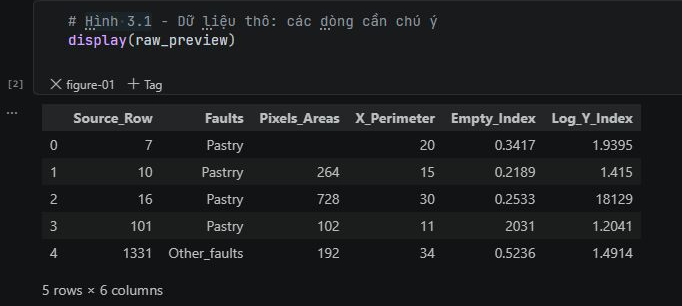
\includegraphics[width=\linewidth]{figures/chuong3/01_du_lieu_tho.png}
  \captionof{figure}{Ảnh cell hiển thị dữ liệu thô trên các dòng nguồn được chọn}
  \label{fig:ch3tho}
\end{minipage}\end{center}

Dữ liệu được tổ chức trong các thư mục tương đối tính từ thư mục gốc của dự án. Thư mục \maCot{data/raw} lưu các nguồn đầu vào; \maCot{data/clean} lưu bảng sau làm sạch; \maCot{data/analysis} lưu bảng đã bổ sung biến phái sinh. Nhật ký xử lý và các bảng kiểm tra được lưu tại \maCot{outputs/buoc_3}; các bảng tổng hợp, hình trực quan và kết quả kiểm thử được tổ chức trong thư mục đầu ra của từng bước tiếp theo. Cách bố trí này giúp đối chiếu các trạng thái dữ liệu và tránh ghi đè nguồn đầu vào.

\section{Thực hiện làm sạch, kết hợp và kiểm chứng dữ liệu}

\subsection{Chuẩn hóa nhãn, kiểu số và loại trùng}

Nhãn được đưa về chữ thường, loại ký tự ngăn cách rồi ánh xạ bằng bảng đã kiểm tra. Chẳng hạn, \maCot{Pastry}, \maCot{Pa stry} và \maCot{Pastrry} cùng được đưa về \maCot{Pastry}; phép ánh xạ xử lý biến thể đã xác nhận, không tự đoán mọi chuỗi gần giống. Quy ước \maCot{K_Scatch} được dùng nhất quán ở bảng phân tích; tên \maCot{K_Scratch} ở nguồn UCI được chuyển theo quy ước này. Mọi nhãn chưa có trong ánh xạ phải được phát hiện trước khi tiếp tục.

Trong đoạn mã sau, \maCot{anh_xa_nhan} là bảng ánh xạ và \maCot{cot_so} là danh sách 27 đặc trưng lấy từ cấu trúc UCI. Khi chuyển kiểu, chuỗi rỗng được xem là thiếu. \maCot{errors="coerce"} chỉ an toàn khi đi cùng kiểm tra thất bại: một chuỗi không rỗng mà không chuyển được không được âm thầm bỏ qua.

\noindent\begin{minipage}{\linewidth}
\setstretch{1}
\begin{lstlisting}[language=Python]
k = du_lieu["Faults"].astype(str).str.lower()
k = k.str.replace(r"[^a-z0-9]", "", regex=True)
du_lieu["Fault_Type_Clean"] = k.map(anh_xa_nhan)
assert du_lieu["Fault_Type_Clean"].notna().all()
for cot in cot_so:
    cu = du_lieu[cot].copy()
    so = pd.to_numeric(cu.mask(cu.eq("")), errors="coerce")
    that_bai = cu.notna() & cu.ne("") & so.isna()
    assert not that_bai.any()
    du_lieu[cot] = so
\end{lstlisting}
\end{minipage}\par

Hình~\ref{fig:ch3chuanhoa} đối chiếu cùng các dòng trước và sau chuẩn hóa. Số biểu diễn nhãn giảm từ 28 về bảy nhãn chuẩn; không có chuỗi số không rỗng nào chuyển đổi thất bại. Những ô vốn trống được giữ là thiếu để xác định căn cứ khôi phục ở bước sau. Trong bảng đối chiếu, \maCot{str} chỉ kiểu chuỗi, \maCot{numeric} chỉ giá trị đã chuyển sang kiểu số; \maCot{NaN} và \maCot{missing} biểu thị giá trị thiếu sau chuyển kiểu.

\begin{center}\begin{minipage}{\linewidth}
  \centering
  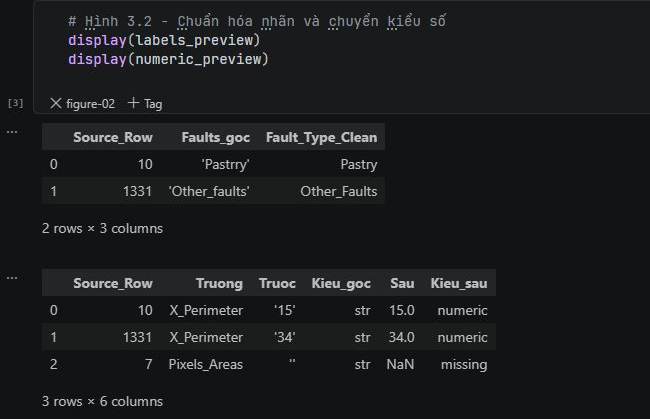
\includegraphics[width=\linewidth]{figures/chuong3/02_chuan_hoa.png}
  \captionof{figure}{Ảnh cell đối chiếu nhãn và kiểu số trước, sau chuẩn hóa}
  \label{fig:ch3chuanhoa}
\end{minipage}\end{center}

Trùng lặp được xác định sau chuẩn hóa theo 27 đặc trưng, ngày gốc và nhãn chuẩn. Chỉ có chung tọa độ chưa đủ để loại một dòng nếu các trường còn lại khác nhau. Mã giữ lần xuất hiện đầu tiên; nhật ký lưu cả \maCot{Source_Row} của dòng loại và \maCot{Kept_Source_Row} của dòng giữ. Cờ \maCot{bi_trung} được tính trước khi lọc để thông tin này không bị mất.

\noindent\begin{minipage}{\linewidth}
\setstretch{1}
\begin{lstlisting}[language=Python]
tieu_chi = cot_so + ["Production_Date", "Fault_Type_Clean"]
bi_trung = du_lieu.duplicated(tieu_chi, keep="first")
du_lieu = du_lieu.loc[~bi_trung].copy()
\end{lstlisting}
\end{minipage}\par

Hình~\ref{fig:ch3trung} minh họa các cặp dòng giữ--loại được ghi trong nhật ký loại trùng. Sau thao tác này, 1.961 dòng còn 1.941 dòng; tổng ô thiếu trong 27 đặc trưng giảm từ 70 xuống 67. Ba ô thiếu không cần điền nữa thuộc các bản sao đã loại, vì vậy số khôi phục không được lấy trực tiếp từ tổng thiếu ban đầu.

\begin{center}\begin{minipage}{\linewidth}
  \centering
  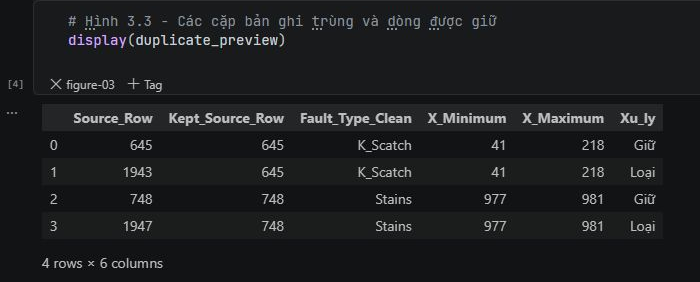
\includegraphics[width=\linewidth]{figures/chuong3/03_loai_trung.png}
  \captionof{figure}{Ảnh cell hiển thị các cặp bản ghi trùng và dòng được giữ}
  \label{fig:ch3trung}
\end{minipage}\end{center}

\subsection{Kiểm tra nội tại trước khôi phục}
\label{sec:ch3kiemtranoitai}

Phép kiểm tra nội tại sử dụng bảng đã chuẩn hóa và loại trùng, trước khi lấy giá trị UCI để điền hoặc sửa. Trong notebook, kiểm tra công thức được thực hiện sau khôi phục. Vì vậy, bài bổ sung một lượt rà soát trên bảng chưa khôi phục để xác định những sai lệch có thể phát hiện từ quan hệ giữa các cột. Các hình và số đếm ở giai đoạn này sử dụng kết quả rà soát bổ sung, được ghi riêng với kết quả đối chiếu nguồn.

Các quan hệ làm việc gồm \maCot{Empty_Index} với diện tích và khung bao, \maCot{Log_Y_Index} với khoảng tọa độ Y, \maCot{LogOfAreas} với diện tích và \maCot{Orientation_Index} với hai kích thước khung bao. Chúng đã được đối chiếu trong quy trình, nhưng không được coi là định nghĩa chính thức do metadata UCI cung cấp. Mã minh họa dưới đây giữ một quan hệ tiêu biểu; \maCot{du_lieu} vẫn là bảng chưa khôi phục.

\noindent\begin{minipage}{\linewidth}
\setstretch{1}
\begin{lstlisting}[language=Python]
dx = du_lieu["X_Maximum"] - du_lieu["X_Minimum"]
dy = du_lieu["Y_Maximum"] - du_lieu["Y_Minimum"]
du_kien = 1 - du_lieu["Pixels_Areas"] / (dx * dy)
du_dieu_kien = du_lieu["Empty_Index"].notna()
du_dieu_kien &= du_kien.notna() & np.isfinite(du_kien)
sai_lech = (du_lieu["Empty_Index"] - du_kien.round(4)).abs()
gan_co = du_dieu_kien & sai_lech.gt(0.00010001)
\end{lstlisting}
\end{minipage}\par

Điều kiện đủ toán hạng và hữu hạn loại khỏi phép kiểm tra những trường hợp chưa tính được giá trị dự kiến. Dung sai xét đến độ chính xác làm tròn của chỉ số. Hình~\ref{fig:ch3noitai} thể hiện giá trị trong tệp và giá trị tính từ những cột cùng dòng; chưa sử dụng giá trị tham chiếu để tạo dấu hiệu phát hiện.

\begin{center}\begin{minipage}{\linewidth}
  \centering
  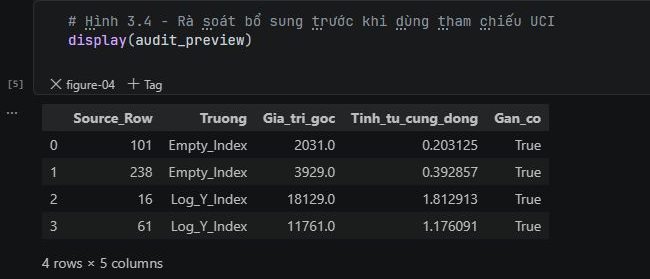
\includegraphics[width=\linewidth]{figures/chuong3/04_kiem_tra_noi_tai.png}
  \captionof{figure}{Ảnh cell kiểm tra nội tại bổ sung trên bảng chưa khôi phục}
  \label{fig:ch3noitai}
\end{minipage}\end{center}

Lượt kiểm tra bổ sung gắn cờ 16 ô: mười ô \maCot{Empty_Index} và sáu ô \maCot{Log_Y_Index}. Một ô có thể vi phạm cả miền giá trị lẫn quan hệ phái sinh; tổng được tính theo cặp dòng--trường duy nhất. Mã chạy lại \maCot{kiem_tra_q0_truoc_tham_chieu.py}, bảng ô vi phạm và bản tóm tắt được lưu tại \maCot{outputs/ra_soat_de_cuong}. Đối chiếu sau khi phát hiện cho thấy 16 cặp dòng--trường này trùng đúng 16 ô trong nhật ký sửa theo UCI. Cờ chỉ xác định vị trí cần xem xét. Giá trị thay thế vẫn phải có căn cứ riêng, được xác nhận khi ghép với nguồn tương ứng.

\subsection{Ghép UCI và khôi phục có truy vết}

Bốn trường \maCot{X_Minimum}, \maCot{X_Maximum}, \maCot{Y_Minimum}, \maCot{Y_Maximum} được chọn làm \maCot{khoa_ghep} sau khi kiểm tra ở cả hai bảng: không thiếu, có giá trị nguyên và không trùng tổ hợp khóa. Bảng \maCot{tham_chieu} chứa 27 đặc trưng, dòng UCI và nhãn suy ra từ bảy cột one-hot; mỗi dòng nguồn phải có đúng một cờ nhãn bằng 1. Các điều kiện này bảo vệ phép ghép khỏi nhân bản bản ghi hoặc chọn nhầm nguồn.

\noindent\begin{minipage}{\linewidth}
\setstretch{1}
\begin{lstlisting}[language=Python]
du_lieu_ghep = du_lieu.merge(
    tham_chieu, on=khoa_ghep, how="left",
    suffixes=("", "_UCI"), validate="one_to_one", indicator=True)
assert du_lieu_ghep["_merge"].eq("both").all()
assert du_lieu_ghep["Fault_Type_Clean"].eq(
    du_lieu_ghep["Fault_Type_UCI"]).all()
\end{lstlisting}
\end{minipage}\par

\maCot{validate="one_to_one"} yêu cầu quan hệ một--một; \maCot{indicator=True} cho phép kiểm tra dòng khớp và chưa khớp~\cite{pandasmerge}. Chỉ khi toàn bộ bản ghi ghép được và nhãn tương ứng nhất quán, giá trị tham chiếu mới được dùng. Hình~\ref{fig:ch3khoiphuc} minh họa ô thiếu và ô có giá trị khác nguồn, cùng vị trí dòng UCI đã xác định.

\begin{center}\begin{minipage}{\linewidth}
  \centering
  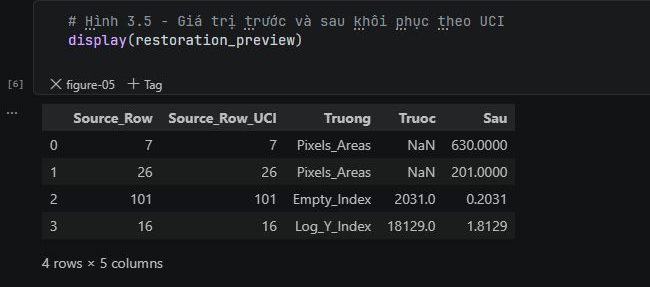
\includegraphics[width=\linewidth]{figures/chuong3/05_khoi_phuc_uci.png}
  \captionof{figure}{Ảnh cell trích nhật ký khôi phục và sửa giá trị theo UCI}
  \label{fig:ch3khoiphuc}
\end{minipage}\end{center}

Hai thao tác được phân biệt trong nhật ký: khôi phục ô đang thiếu và sửa ô có giá trị khác nguồn. Ví dụ, \maCot{Pixels_Areas} tại dòng nguồn 7 được khôi phục thành 630; \maCot{Empty_Index} tại dòng 101 được sửa từ 2031 thành 0,2031. Giá trị sau lấy từ UCI tại khóa đã ghép, không suy đoán bằng cách dịch dấu thập phân. Đoạn mã sau minh họa một trường \maCot{cot} không thuộc khóa; mã đầy đủ bổ sung loại thao tác và căn cứ trước khi ghép nhật ký của các trường.

\noindent\begin{minipage}{\linewidth}
\setstretch{1}
\begin{lstlisting}[language=Python]
cu = du_lieu_ghep[cot].copy()
moi = du_lieu_ghep[cot + "_UCI"]
thieu = cu.isna()
khac = ~thieu & ~np.isclose(cu, moi, rtol=0, atol=1e-9)
doi = thieu | khac
nhat_ky = du_lieu_ghep.loc[doi,
    ["Source_Row", "Source_Row_UCI"]].copy()
nhat_ky["Truong"] = cot
nhat_ky["Gia_tri_truoc"] = cu[doi]
nhat_ky["Gia_tri_sau"] = moi[doi]
du_lieu_ghep.loc[doi, cot] = moi[doi]
\end{lstlisting}
\end{minipage}\par

Quy trình khôi phục 67 ô thiếu và sửa 16 giá trị số. Các ví dụ ở Hình~\ref{fig:ch3khoiphuc} được trích từ nhật ký khôi phục ô thiếu và nhật ký sửa giá trị; mỗi mục ghi dòng nguồn, dòng tham chiếu, trường thay đổi và giá trị trước--sau. Sau xử lý, 52.407 ô đặc trưng được đối chiếu với nguồn tham chiếu. Độ khớp này xác nhận đúng phép ghép và thao tác khôi phục; do UCI đã cung cấp giá trị thay thế, nó không phải thước đo độc lập về khả năng phát hiện sai sót. Nhật ký phát hiện trước tham chiếu và nhật ký thay đổi được giữ riêng để kiểm tra hai hoạt động này.

\subsection{Chuẩn hóa ngày, gắn cờ diện tích và kiểm tra đầu ra}

Ngày gốc được giữ trong \maCot{Production_Date}; ngày chuẩn lưu ở \maCot{Production_Date_Clean}, kèm cờ \maCot{Date_Is_Simulated} để nhận biết ngày mô phỏng. Hàm \maCot{clean_simulated_date} chuẩn hóa các cách biểu diễn ngày theo lịch mô phỏng gồm các ngày 2, 3, 10, 21 và 30 tháng 11 năm 2025. Ví dụ, giá trị đầu vào tại dòng 2 là 2025-02-11 được chuyển thành 2025-11-02 theo lịch đã biết. Đây là quy tắc riêng của dữ liệu thực hành, không phải cách đảo ngày/tháng áp dụng cho mọi dữ liệu. Chuẩn hóa phục vụ tính nhất quán và truy vết; ngày này không được dùng để phân tích xu hướng sản xuất.

\noindent\begin{minipage}{\linewidth}
\setstretch{1}
\begin{lstlisting}[language=Python]
du_lieu_ghep["Production_Date_Clean"] = pd.to_datetime(
    du_lieu_ghep["Production_Date"].map(clean_simulated_date))
du_lieu_ghep["Date_Is_Simulated"] = True
area = du_lieu_ghep["Pixels_Areas"]
q1, q3 = area.quantile([0.25, 0.75])
du_lieu_ghep["Area_Outlier_Flag"] = (
    area.lt(q1 - 1.5 * (q3 - q1)) | area.gt(q3 + 1.5 * (q3 - q1)))
\end{lstlisting}
\end{minipage}\par

Cờ diện tích được tính trên toàn bộ 1.941 dòng đã khôi phục theo hàng rào $1{,}5\times\mathrm{IQR}$. Có 395 dòng được gắn cờ và giữ lại. Cờ toàn tập này phục vụ xem xét dữ liệu; các điểm ngoài râu ở boxplot Q5 được tính lại trong từng nhóm, nên hai số đếm không đồng nghĩa. Theo nguyên tắc ở Chương 1, diện tích lớn chưa đủ căn cứ xác định sai dữ liệu~\cite{nistbox}.

Trước khi xuất bảng sau làm sạch, quy trình kiểm tra số dòng, nhãn hợp lệ, không thiếu đặc trưng, cờ dòng thép, quan hệ tọa độ, miền độ sáng và các công thức làm việc. Bảng được lưu ở định dạng CSV rồi đọc lại để đối chiếu dữ liệu số và nhãn; ngày được phân tích về kiểu ngày khi cần so sánh. Tùy chọn \maCot{index=False} tránh xuất thêm chỉ số dòng của DataFrame; mã hóa \maCot{utf-8-sig} hỗ trợ lưu chữ tiếng Việt. Kiểm tra sau xuất bảo đảm bảng giao cho bước phân tích giữ đúng giá trị đã xử lý.

\section{Tạo biến phái sinh và các bảng thống kê}

Bảng phân tích được tạo từ bản sao bảng sau làm sạch. Trong mã minh họa, \maCot{loi_thep_sach} đại diện cho bảng sau làm sạch và \maCot{d} là tên viết gọn của bảng phân tích. Trước khi tổng hợp cột dòng thép \maCot{Steel_Type}, hai cờ A300/A400 được kiểm tra chỉ nhận 0 hoặc 1 và có tổng bằng 1 trên mỗi dòng. Kích thước, diện tích và độ dày phải dương; độ sáng tối đa không được nhỏ hơn tối thiểu. Những điều kiện này cần đạt trước khi lấy hiệu hoặc logarit.

\noindent\begin{minipage}{\linewidth}
\setstretch{1}
\begin{lstlisting}[language=Python]
d = loi_thep_sach.copy(deep=True)
d["Steel_Type"] = np.where(
    d["TypeOfSteel_A300"].eq(1), "A300", "A400")
d["X_Range"] = d["X_Maximum"] - d["X_Minimum"]
d["Y_Range"] = d["Y_Maximum"] - d["Y_Minimum"]
d["Luminosity_Range"] = (
    d["Maximum_of_Luminosity"] - d["Minimum_of_Luminosity"])
d["Log_Pixels_Areas"] = np.log10(d["Pixels_Areas"].astype(float))
\end{lstlisting}
\end{minipage}\par

Hình~\ref{fig:ch3phantich} minh họa các trường bổ sung trên những bản ghi thực tế, cùng ngày chuẩn và cờ mô phỏng. \maCot{X_Range} và \maCot{Y_Range} mô tả kích thước khung bao, không thay thế diện tích vùng lỗi. \maCot{Luminosity_Range} là hiệu độ sáng tối đa--tối thiểu; chưa có căn cứ đồng nhất nó với \maCot{Luminosity_Index}. \maCot{Log_Pixels_Areas} dùng cơ số 10 và tính lại thông tin đã có trong \maCot{LogOfAreas}; sai khác được kiểm tra trong dung sai 0,00010001 do làm tròn. Cột này hỗ trợ kiểm chứng, không tăng số đặc trưng độc lập.

\begin{center}\begin{minipage}{\linewidth}
  \centering
  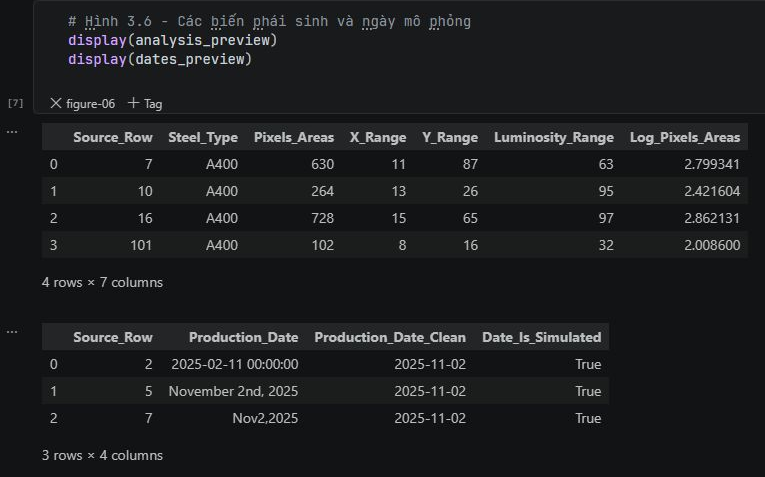
\includegraphics[width=\linewidth]{figures/chuong3/06_du_lieu_phan_tich.png}
  \captionof{figure}{Ảnh cell hiển thị biến phái sinh và ngày mô phỏng sau chuẩn hóa}
  \label{fig:ch3phantich}
\end{minipage}\end{center}

Các bảng thống kê được tính trực tiếp từ bảng phân tích. Q1 dùng số đếm giảm dần, tỷ trọng và lũy kế. Q2 bắt đầu từ bảng chéo nhãn--dòng thép; chuẩn hóa theo cột cho cơ cấu nhãn trong dòng thép, chuẩn hóa theo hàng cho phân bố dòng thép trong từng nhãn. Hai tỷ trọng được lưu thành hai trường riêng trong bảng thống kê; mã minh họa dưới đây thể hiện phép chia theo hai chiều.

\noindent\begin{minipage}{\linewidth}
\setstretch{1}
\begin{lstlisting}[language=Python]
dem = pd.crosstab(d["Fault_Type_Clean"], d["Steel_Type"])
trong_dong_thep = dem.div(dem.sum(axis=0), axis=1) * 100
trong_nhan = dem.div(dem.sum(axis=1), axis=0) * 100
g = d.groupby("Fault_Type_Clean")["Pixels_Areas"]
thong_ke = g.agg(N="count", Median="median", SD="std")
thong_ke["P25"] = g.quantile(0.25)
thong_ke["P75"] = g.quantile(0.75)
thong_ke["IQR"] = thong_ke["P75"] - thong_ke["P25"]
\end{lstlisting}
\end{minipage}\par

Mã minh họa thống kê diện tích được áp dụng tương tự cho độ sáng và độ dày; bổ sung min/max khi xuất bảng. Độ dày còn được nhóm theo nhãn và dòng thép để so sánh trong cùng nhãn. \maCot{std} sử dụng độ lệch chuẩn mẫu với mẫu số $N-1$; nhóm $N=1$ giữ kết quả chưa xác định, không điền 0. Với dashboard, dòng thép không có quan sát sau lọc cũng chưa có tỷ trọng. Bảng thống kê và biểu đồ đều phải giữ cỡ mẫu tương ứng với phạm vi đang xét.

\section{Xây dựng biểu đồ theo câu hỏi phân tích}

Biểu đồ được dựng từ bảng phân tích và các bảng tổng hợp đã kiểm tra, không tính lại trên nguồn thô. Ba hình dưới đây minh họa trực tiếp cách chuyển số liệu thành biểu đồ cơ cấu, quan hệ giữa hai biến và phân bố theo nhóm. Mã được rút gọn để làm rõ thao tác chính; tiêu đề, nhãn trục, cỡ mẫu, màu và chú thích nguồn được bổ sung trong mã đầy đủ. \maCot{MAU_LOI} là bảng màu gắn cố định với bảy nhãn, được dùng thống nhất giữa các hình.

Những hình còn lại được tổ chức theo cùng nguyên tắc. Q2 dùng số đếm cho cột nhóm, còn cột 100\% dùng tỷ trọng trong từng dòng thép; bảng tỷ trọng trong nhãn cung cấp căn cứ đọc ngưỡng trên 90\%. Q4 dùng boxplot độ dày và bảng nhãn--dòng thép. Mỗi hình phải ghi rõ phạm vi và giữ cỡ mẫu khi so sánh.

\subsection{Biểu đồ cơ cấu và tỷ trọng lũy kế}

Thanh ngang và Pareto ở Q1 cùng sử dụng thứ tự số đếm giảm dần. Trong Pareto, cột biểu diễn số bản ghi, còn đường biểu diễn tỷ trọng lũy kế trên tổng bản ghi lỗi. Hai đại lượng dùng hai trục tung riêng. Mốc 80\% được vẽ ở trục phần trăm để đọc mức tập trung trong mẫu.

\noindent\begin{minipage}{\linewidth}
\setstretch{1}
\begin{lstlisting}[language=Python]
dem = d["Fault_Type_Clean"].value_counts()
luy_ke = dem.cumsum() / dem.sum() * 100
fig, ax = plt.subplots(figsize=(11, 6))
ax.bar(dem.index, dem, color=[MAU_LOI[n] for n in dem.index])
ax_luy_ke = ax.twinx()
ax_luy_ke.plot(dem.index, luy_ke, marker="o", color="black")
ax_luy_ke.axhline(80, linestyle="--", color="gray")
ax_luy_ke.set_ylim(0, 105)
\end{lstlisting}
\end{minipage}\par

Hình~\ref{fig:ch3pareto} là sản phẩm từ mã vẽ đầy đủ trên 1.941 bản ghi sau xử lý. Nhãn phần trăm nằm trên đường lũy kế; tên loại lỗi được xoay để tránh chồng chữ. Chú thích phân biệt số lượng với phần trăm, giúp người đọc theo dõi đúng mẫu số khi đối chiếu bảng cơ cấu.

\begin{center}\begin{minipage}{\linewidth}
  \centering
  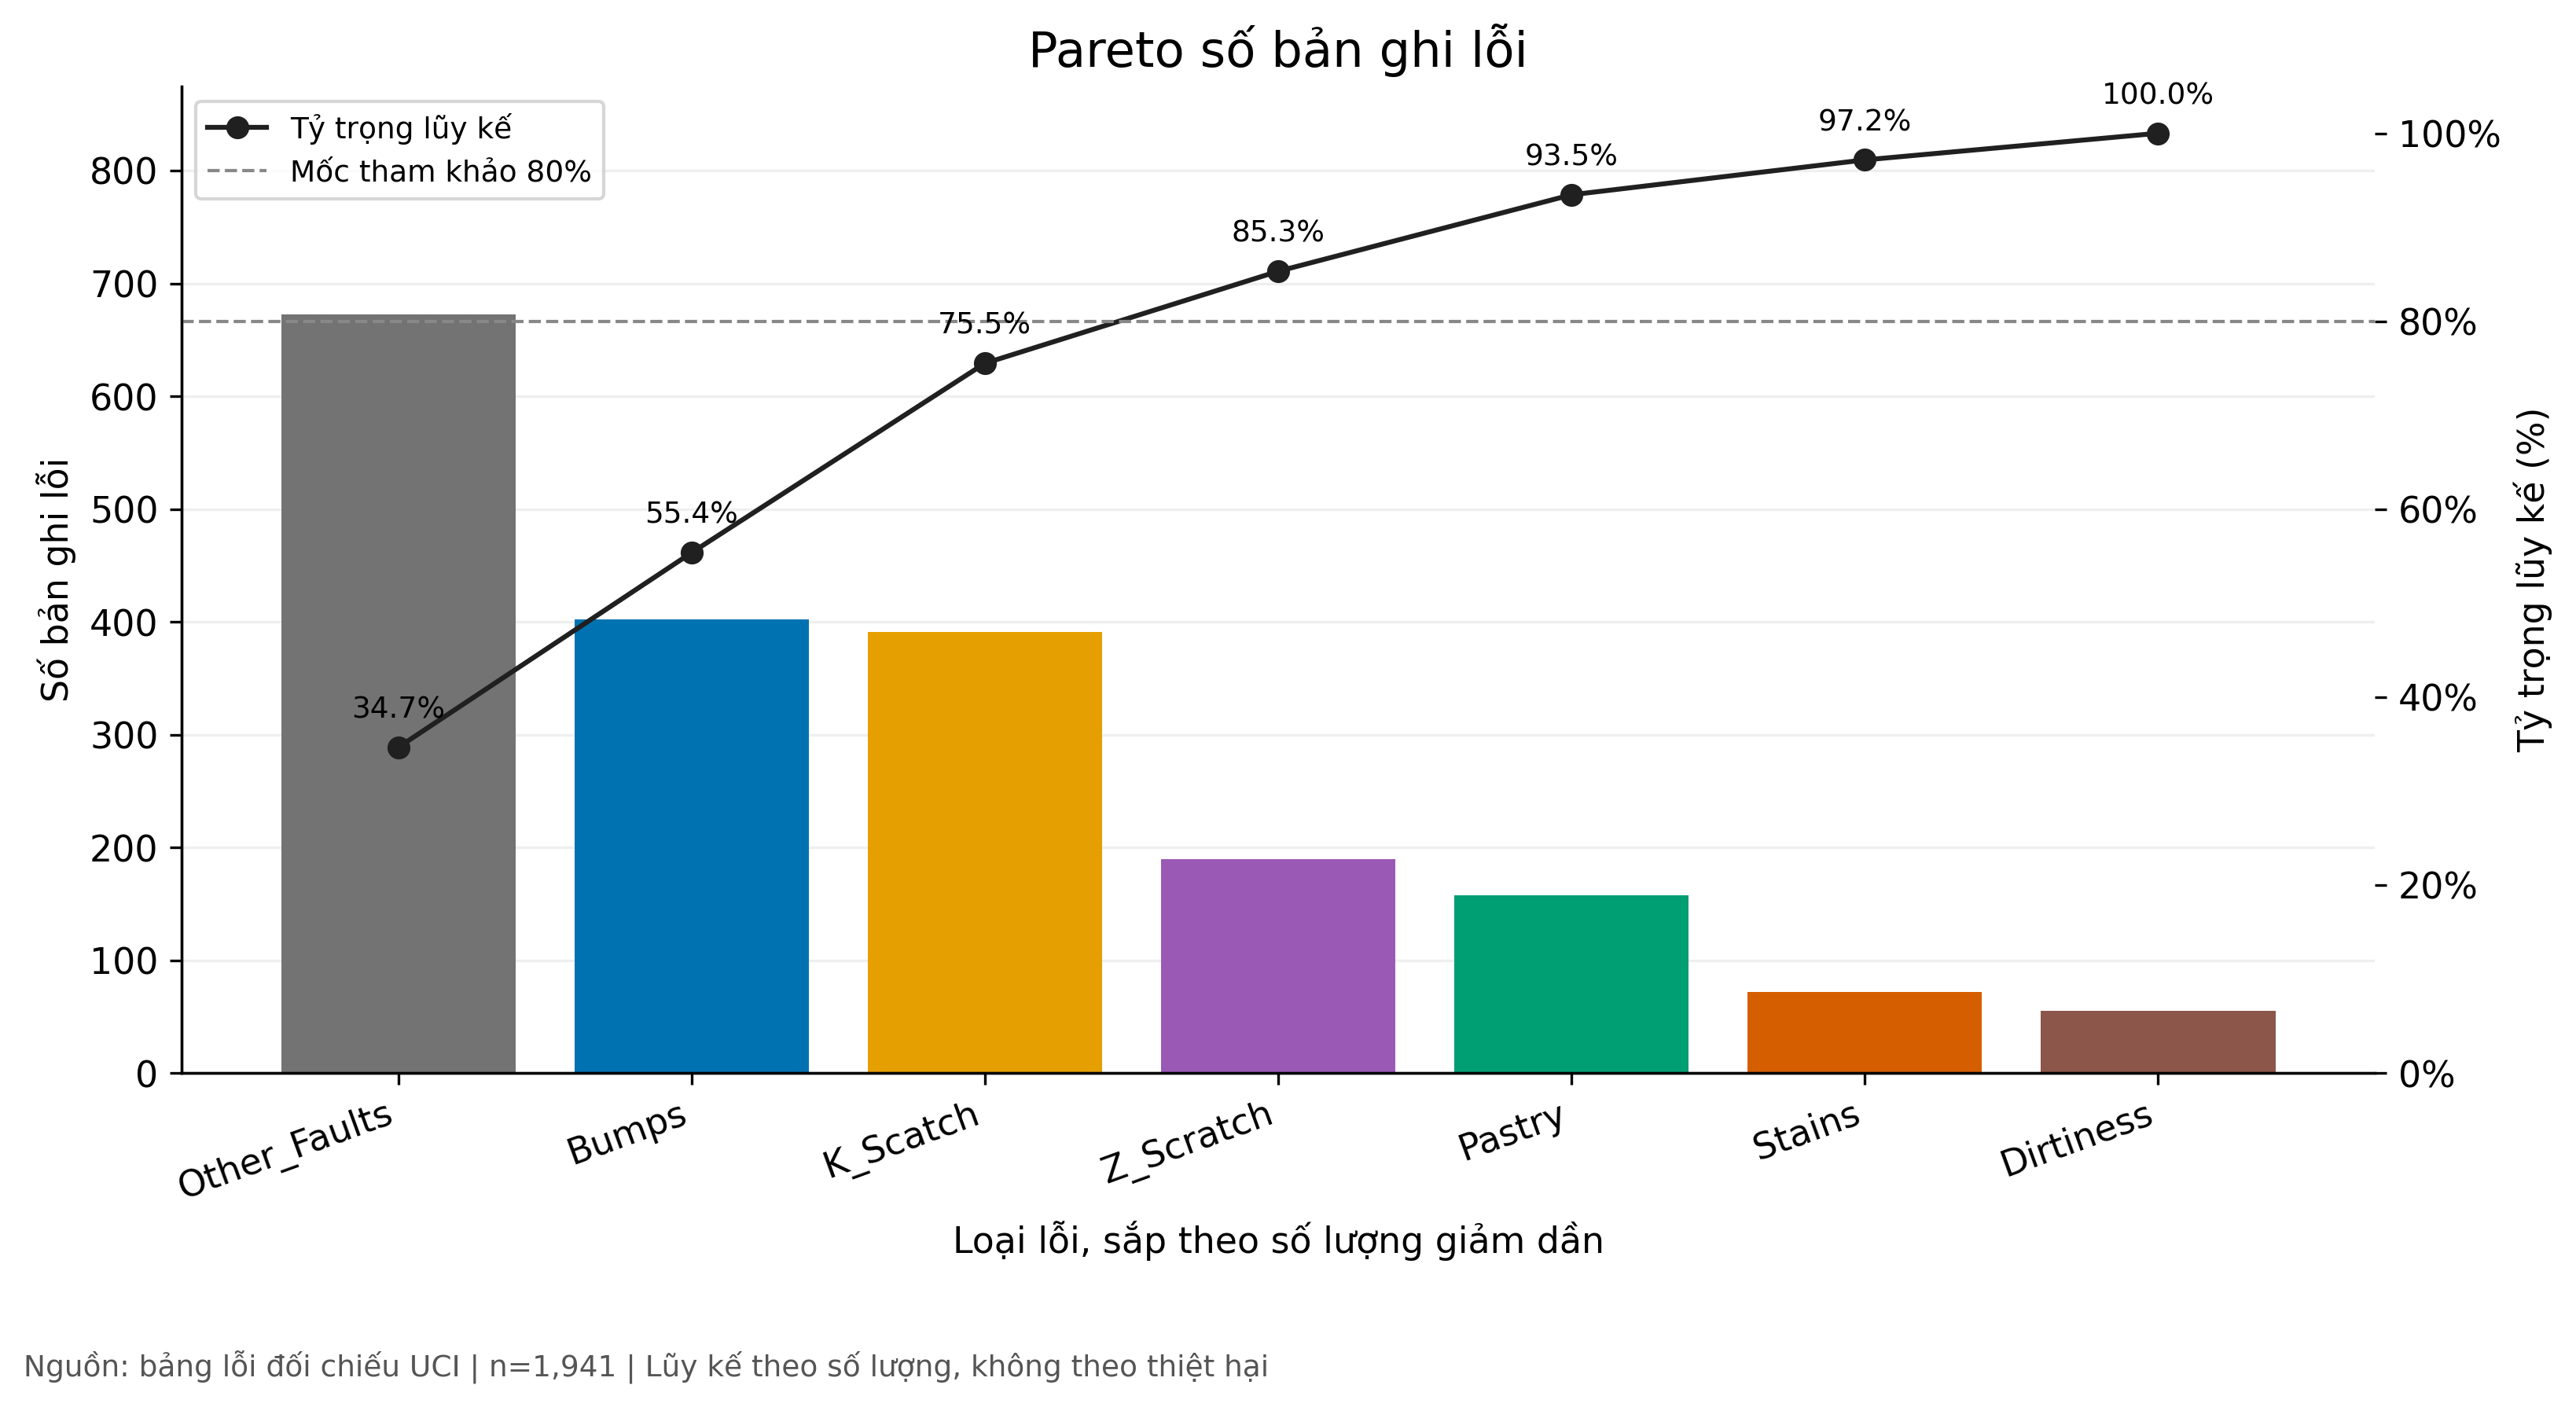
\includegraphics[width=\linewidth]{figures/chuong3/07_pareto_loi.png}
  \captionof{figure}{Minh họa Pareto từ bảng số đếm và tỷ trọng lũy kế của các nhãn lỗi}
  \label{fig:ch3pareto}
\end{minipage}\end{center}

\subsection{Biểu đồ phân tán độ sáng theo nhãn}

Q3 đặt độ sáng tối thiểu trên trục ngang và tối đa trên trục dọc. Mỗi bản ghi tạo một điểm; nhóm nhãn quyết định màu. Tham số \maCot{alpha=0.35} giảm độ đậm để các vùng có nhiều điểm chồng lên nhau vẫn đọc được. Không nối các điểm, vì dữ liệu không biểu diễn một chuỗi có thứ tự.

\noindent\begin{minipage}{\linewidth}
\setstretch{1}
\begin{lstlisting}[language=Python]
fig, ax = plt.subplots(figsize=(11, 7))
for nhan, nhom in d.groupby("Fault_Type_Clean"):
    ax.scatter(
        nhom["Minimum_of_Luminosity"],
        nhom["Maximum_of_Luminosity"],
        s=22, alpha=0.35, color=MAU_LOI[nhan],
        edgecolors="none", label=f"{nhan} (n={len(nhom)})")
ax.legend(title="Loai loi", bbox_to_anchor=(1.02, 1))
\end{lstlisting}
\end{minipage}\par

Hình~\ref{fig:ch3scatter} giữ toàn bộ bản ghi, ghi cỡ mẫu từng nhãn trong chú giải và sử dụng thang độ sáng theo nguồn. Hệ số Pearson trong tiêu đề là thông tin bổ trợ về quan hệ giữa hai biến. Nhận xét vùng trung tâm cần đối chiếu thêm P25/P75 theo tiêu chí tại mục~\ref{sec:yeucauphanTich}, vì độ trong suốt và sự chồng điểm chưa thay thế được bảng thống kê.

\begin{center}\begin{minipage}{\linewidth}
  \centering
  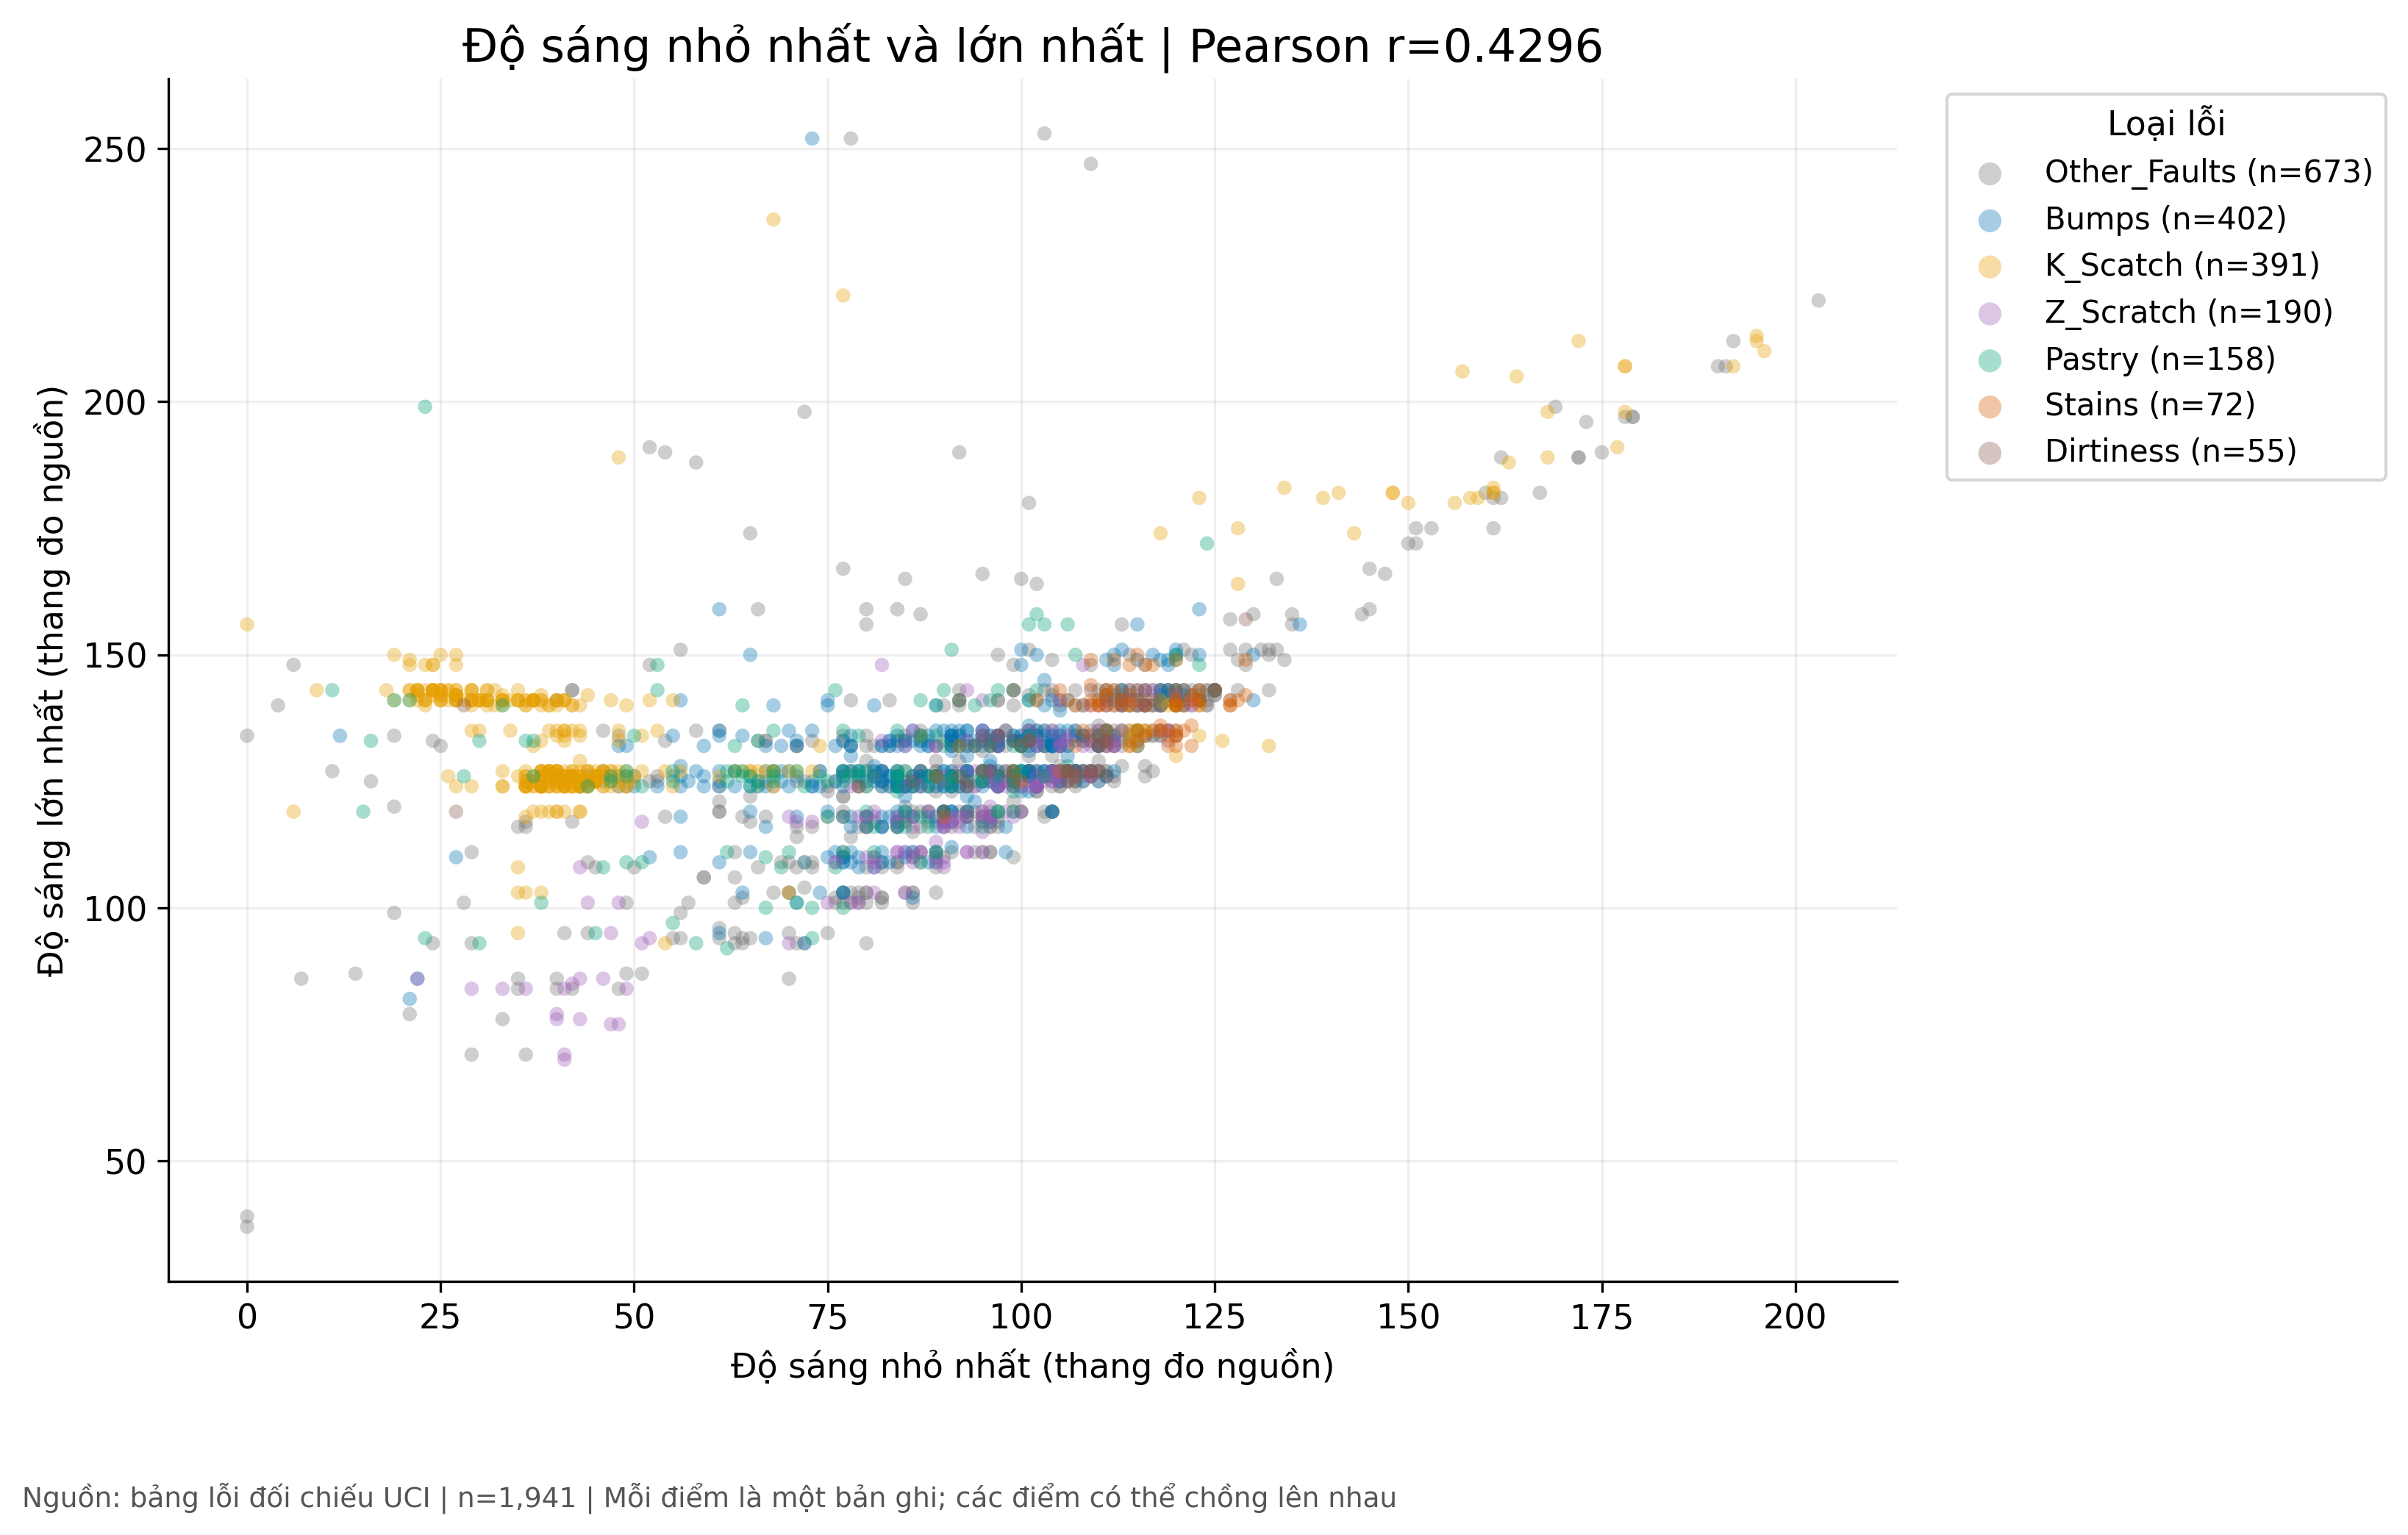
\includegraphics[width=\linewidth]{figures/chuong3/08_scatter_do_sang.png}
  \captionof{figure}{Minh họa scatter độ sáng tối thiểu--tối đa, phân biệt nhãn bằng màu và cỡ mẫu}
  \label{fig:ch3scatter}
\end{minipage}\end{center}

\subsection{Boxplot diện tích trên trục logarit}

Q5 giữ diện tích gốc để tính hộp, râu và điểm ngoài râu, sau đó mới đổi trục hiển thị sang log. Các nhãn được xếp cùng thứ tự với bảng cơ cấu; hộp nằm ngang để đọc rõ tên nhóm và cỡ mẫu. Điều kiện diện tích dương đã được kiểm tra ở bước tạo bảng phân tích.

\noindent\begin{minipage}{\linewidth}
\setstretch{1}
\begin{lstlisting}[language=Python]
nhan = d["Fault_Type_Clean"].value_counts().index.tolist()
mau = [d.loc[d["Fault_Type_Clean"].eq(n), "Pixels_Areas"]
       for n in nhan]
fig, ax = plt.subplots(figsize=(10, 5))
ax.boxplot(mau, vert=False, whis=1.5, showfliers=True)
ax.set_yticks(range(1, len(nhan) + 1), nhan)
ax.invert_yaxis()
ax.set_xscale("log")
\end{lstlisting}
\end{minipage}\par

Hình~\ref{fig:ch3boxarea} là đầu ra hoàn chỉnh tương ứng với đoạn mã minh họa. \maCot{set_xscale("log")} thay cách hiển thị sau khi hộp đã được tính từ \maCot{Pixels_Areas}; nó không thay dữ liệu đầu vào thành cột logarit. Nhãn trục vẫn ghi diện tích gốc. Các điểm ngoài râu được giữ và tính theo từng nhãn, khác với cờ IQR toàn tập ở bước làm sạch.

\begin{center}\begin{minipage}{\linewidth}
  \centering
  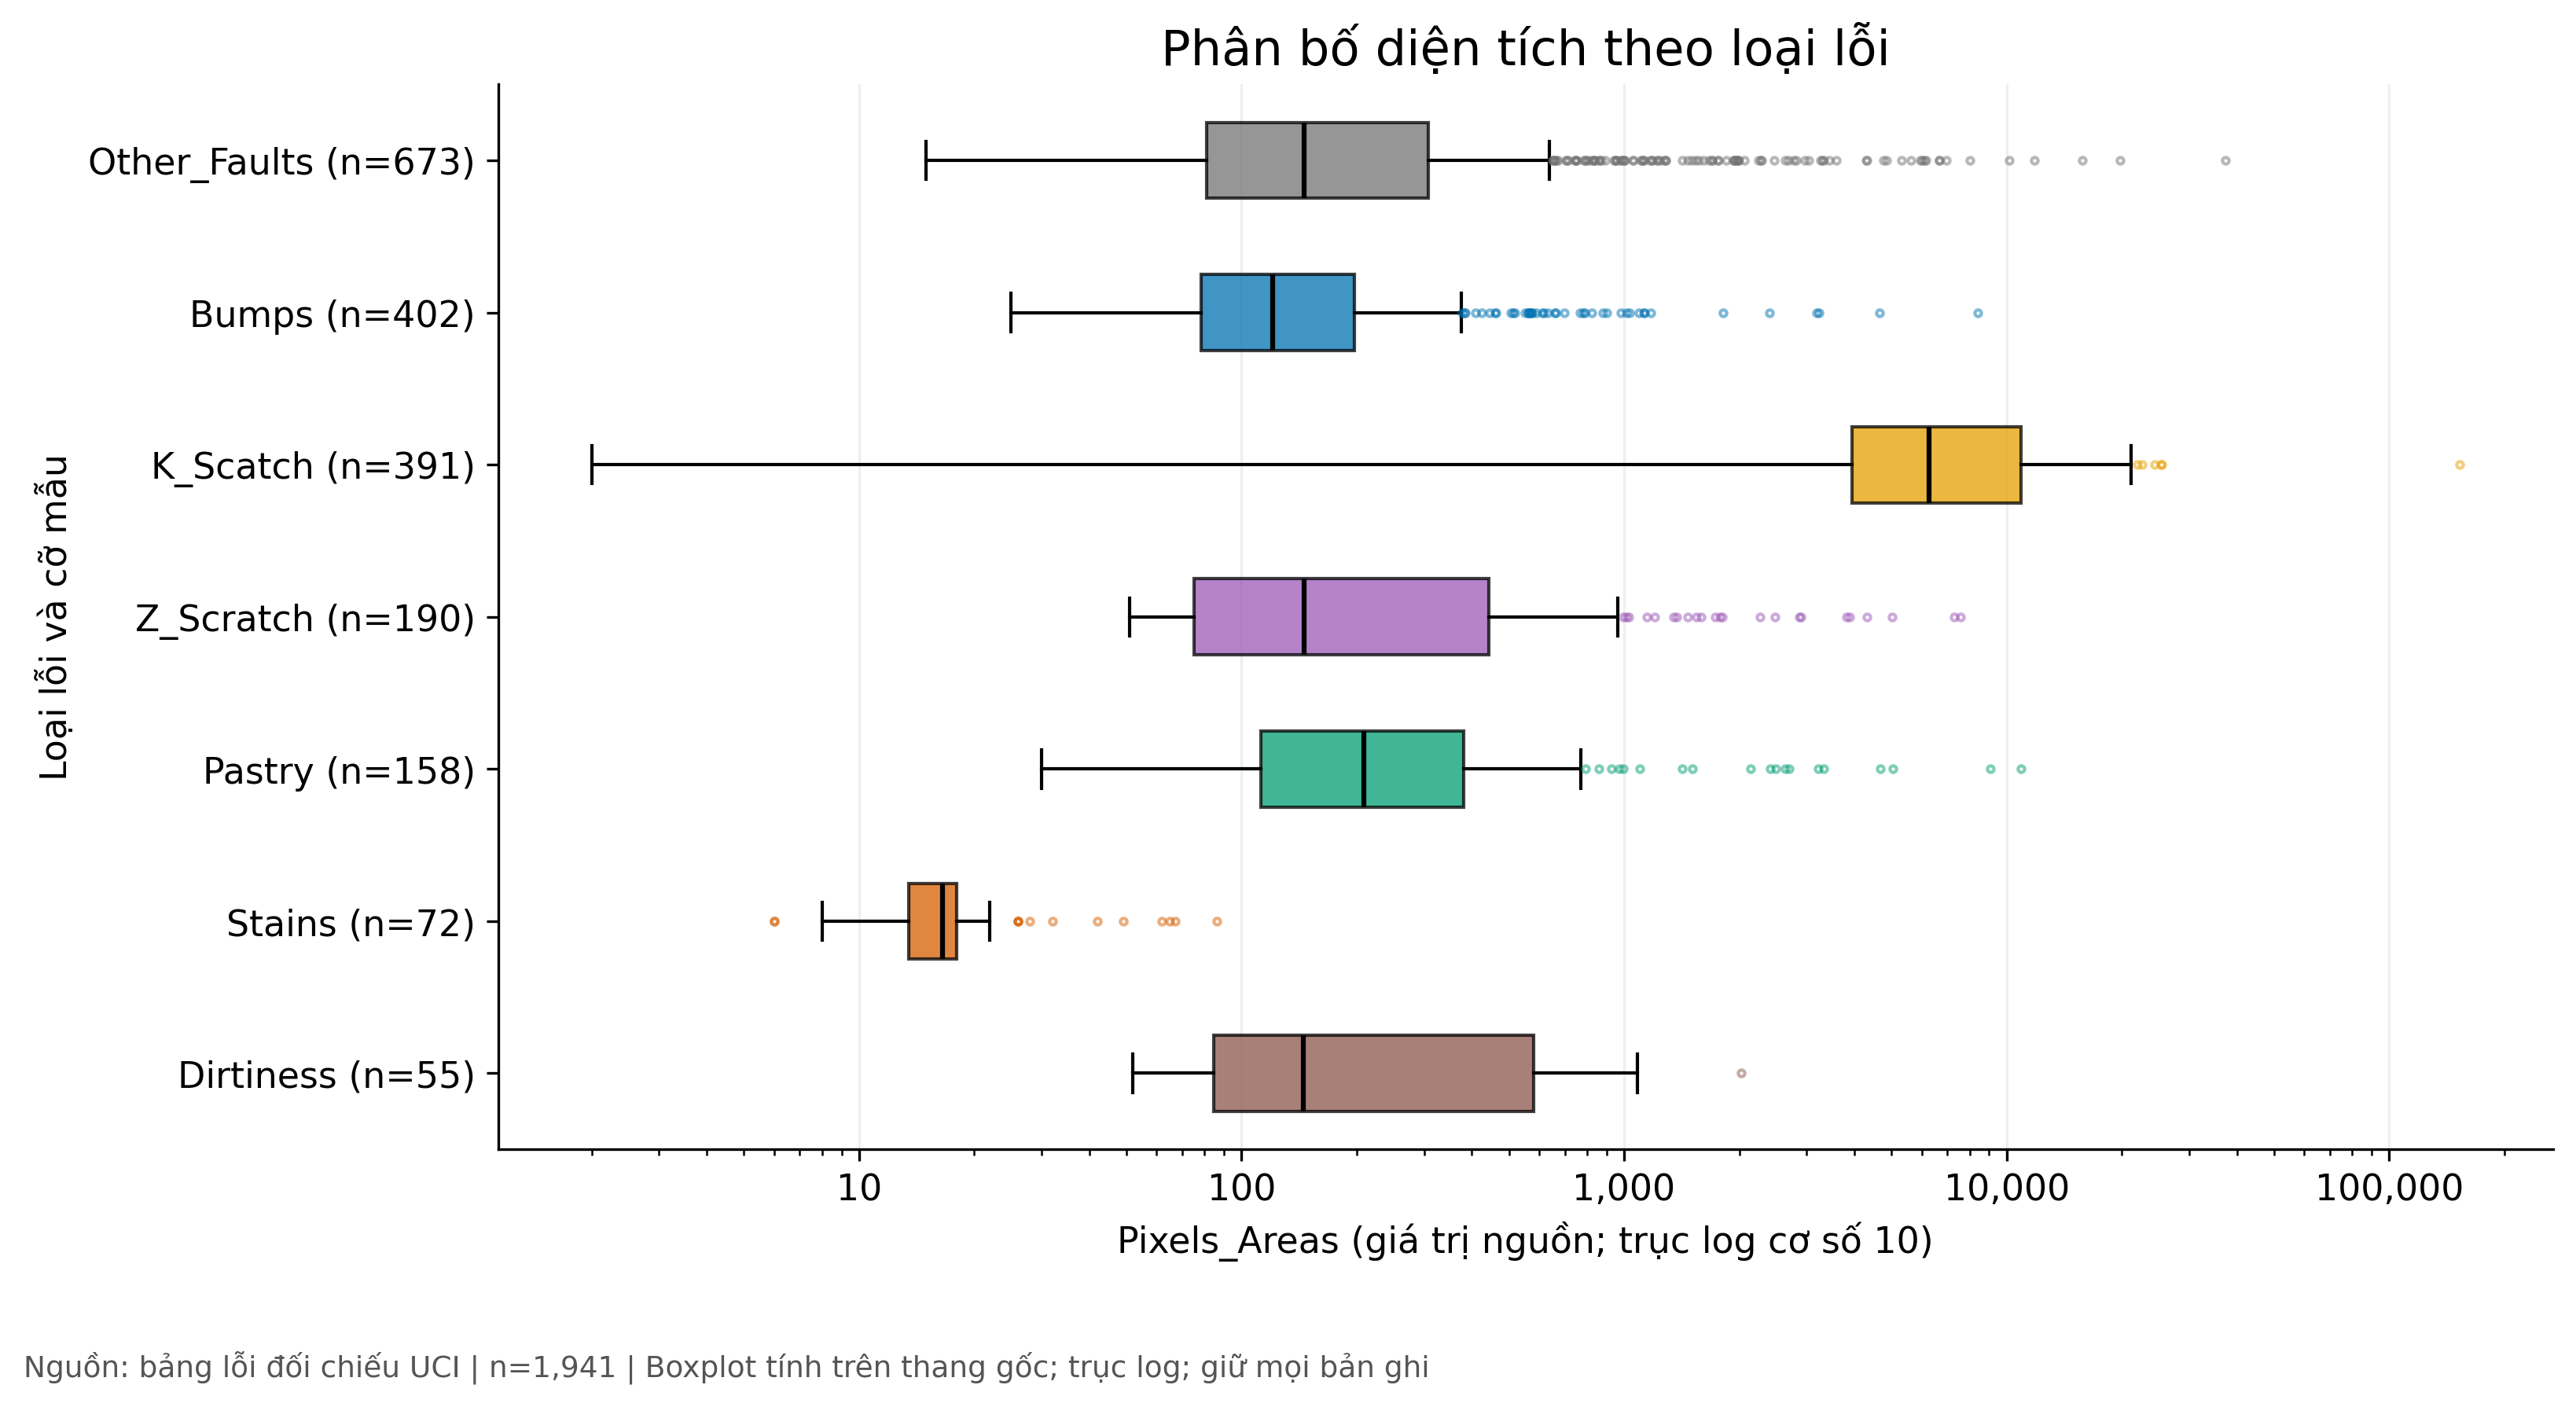
\includegraphics[width=\linewidth]{figures/chuong3/09_boxplot_dien_tich_log.png}
  \captionof{figure}{Minh họa boxplot tính trên diện tích gốc rồi hiển thị với trục log cơ số 10}
  \label{fig:ch3boxarea}
\end{minipage}\end{center}

Các hình được xuất PNG độ phân giải 300 dpi và SVG để có thể đưa vào báo cáo với chữ rõ~\cite{matplotlib}. Bảng hỗ trợ được xuất CSV cùng giai đoạn, giúp đối chiếu hình với số liệu. Các minh họa ở mục này thể hiện cách dựng và quy tắc hiển thị; phần trả lời đầy đủ Q1--Q5 được triển khai ở Chương 4.

\section{Xây dựng dashboard tương tác}

\subsection{Kiến trúc và tổ chức giao diện}

Dashboard dùng Streamlit để tổ chức giao diện và Plotly để vẽ biểu đồ tương tác. Khi đọc nguồn, mô-đun xử lý tái lập quy trình làm sạch và tạo biến từ bảng thực hành cùng bảng tham chiếu UCI. Kết quả hợp lệ được giữ trong một bản dữ liệu cùng thông tin chất lượng và thời điểm kiểm tra. Dashboard không chỉnh trực tiếp dữ liệu gốc khi người dùng thao tác bộ lọc.

\begin{center}\begin{minipage}{\linewidth}
  \centering
  \begingroup
  \small
  \setstretch{1.05}
  \setlength{\fboxsep}{6pt}
  \fbox{\parbox{0.88\linewidth}{\centering
  \textbf{Đọc nguồn và kiểm tra} $\longrightarrow$ \textbf{Bản dữ liệu hợp lệ}\\[5pt]
  $\downarrow$\\[5pt]
  \textbf{Áp dụng bộ lọc lỗi} $\longrightarrow$ \textbf{Tập con đang chọn}\\[5pt]
  $\downarrow$\\[5pt]
  \textbf{KPI -- biểu đồ -- bảng thống kê -- CSV}\\[5pt]
  Tab chất lượng đọc thông tin toàn nguồn từ bản dữ liệu hợp lệ.
  }}
  \endgroup
  \captionof{figure}{Luồng dữ liệu trong phần phân tích lỗi của dashboard}
  \label{fig:ch3dashboardflow}
\end{minipage}\end{center}

Giao diện có ba tab: phân tích lỗi thép, bối cảnh ngành và dữ liệu--chất lượng. Tab chất lượng cho biết toàn bộ nguồn có đáp ứng điều kiện xử lý hay không. Tab bối cảnh sử dụng UN Comtrade độc lập, có bộ lọc năm riêng; đây là chức năng bổ sung, không ghép thương mại với từng bản ghi lỗi. Hình~\ref{fig:ch3dashboardflow} thể hiện luồng của phần phân tích chính.

\subsection{Bộ lọc, KPI, biểu đồ và bảng dữ liệu}

Ba bộ lọc chính chọn dòng thép, nhãn và khoảng độ dày. Kết quả lọc được lưu thành một bảng \maCot{selected}; số bản ghi, số nhãn, trung vị diện tích, trung vị độ dày và các biểu đồ đều tính từ bảng này. Đoạn mã dưới đây rút gọn thao tác trong mô-đun xử lý; \maCot{steels}, \maCot{labels} và \maCot{thickness} nhận giá trị từ giao diện.

\noindent\begin{minipage}{\linewidth}
\setstretch{1}
\begin{lstlisting}[language=Python]
chon = (data["Steel_Type"].isin(steels)
    & data["Fault_Type_Clean"].isin(labels)
    & data["Steel_Plate_Thickness"].between(*thickness))
selected = data.loc[chon].copy()
n = len(selected)
median_area = selected["Pixels_Areas"].median()
csv = selected.to_csv(index=False).encode("utf-8-sig")
\end{lstlisting}
\end{minipage}\par

Khi tập con rỗng, dashboard thông báo không có bản ghi phù hợp; các trung vị hiển thị dấu gạch thay vì 0. Người dùng có thể mở rộng phạm vi hoặc đặt lại bộ lọc. Bảng hỗ trợ và CSV trong phần lỗi dùng đúng tập con, còn các chỉ số chất lượng ghi rõ phạm vi toàn nguồn. Cách tổ chức này giúp kiểm thử một thao tác lọc bằng cách đối chiếu số dòng, KPI, hình và tệp tải về.

\subsection{Cập nhật nguồn và xử lý lỗi}

Nút làm mới đọc lại nguồn và kiểm tra trước khi thay bản dữ liệu đang hiển thị. Chế độ tự động đọc lại mỗi năm phút sử dụng \maCot{st.fragment}; thay đổi bộ lọc chỉ tính và vẽ lại từ bản đang giữ, không kích hoạt đọc tệp cho từng thao tác. Trạng thái bộ lọc được rà soát khi nguồn thay đổi để loại lựa chọn không còn hợp lệ. Cách dùng trạng thái phù hợp với cơ chế widget của Streamlit~\cite{streamlit}.

Nếu nguồn mới không đạt điều kiện, ứng dụng giữ bản hợp lệ gần nhất và hiển thị lỗi cùng thời điểm bản đó được kiểm tra. Khi chưa có bản trong phiên, chương trình có thể đọc bản đã lưu; nếu vẫn không có dữ liệu hợp lệ, giao diện dừng phần phân tích và báo nguyên nhân. Cơ chế này tránh để dữ liệu chưa kiểm chứng thay thế kết quả đang xem.

Với chức năng thương mại bổ sung, gọi API là lựa chọn riêng. Bộ nhớ đệm có thời hạn 15 phút; nút làm mới chủ động xóa đệm khi người dùng chọn gọi lại API. Chu kỳ năm phút là đọc lại tệp hoặc nguồn được cấu hình, chưa phải thu nhận cảm biến thời gian thực. Thời điểm kiểm tra nguồn cũng độc lập với \maCot{Production_Date_Clean} mô phỏng.

\section{Tổ chức thực thi và tiểu kết}

Notebook được thực thi tuần tự; bước sau chỉ sử dụng bảng đã đạt điều kiện kiểm tra của bước trước. Bảng trung gian, nhật ký và dữ liệu xuất được giữ để đối chiếu khi chạy lại. Kiểm tra nội tại trước khôi phục là lượt rà soát bổ sung đã mô tả ở mục~\ref{sec:ch3kiemtranoitai}. Dashboard được chạy trong môi trường Python, sử dụng mô-đun xử lý để tái lập bảng dữ liệu trước khi hiển thị.

Các hình trung gian và đoạn mã cho phép theo dõi dữ liệu từ biểu diễn thô đến bảng phân tích, đồng thời xác định căn cứ của từng thay đổi. Chương 4 trình bày kết quả Q0--Q5, giao diện thực tế và minh chứng kiểm thử từ những đầu ra này.

% ===== END: chuong/chuong3 =====
% ===== BEGIN: chuong/chuong4 =====
% Bảy biểu đồ từ output notebook bước 1--6 và một ảnh chụp dashboard thực tế.
\chapter{Kết quả phân tích, kiểm thử và thảo luận}
\label{chap:ketqua}

Từ 1.941 bản ghi lỗi đã làm sạch, chương này đi từ cơ cấu chung đến đặc điểm của từng nhóm. Hai nhãn \maCot{Bumps} và \maCot{K_Scatch} có số lượng gần bằng nhau, nhưng phân bố theo dòng thép, độ sáng, độ dày và diện tích cho thấy những khác biệt đáng chú ý. Việc lần lượt xem các chiều này giúp chuyển một thứ hạng tần suất thành mô tả cụ thể để lựa chọn nội dung cần kiểm chứng tiếp.

Mạch phân tích gồm Q0 xác nhận dữ liệu đầu vào; Q1 mô tả mức tập trung của nhãn; Q2 xác định phân bố theo dòng thép; Q3--Q5 bổ sung đặc điểm độ sáng, độ dày và diện tích. Bảy biểu đồ phân tích đều xuất hiện dưới các ô mã đã chạy của notebook \maCot{buoc_1_2_3_4_5_6_loi_be_mat_thep.ipynb}. Tên mục và mã hình trong notebook được ghi dưới mỗi biểu đồ để đối chiếu khi số thứ tự ô thay đổi. Đơn vị phân tích xuyên suốt là một bản ghi được gán nhãn lỗi; các tỷ trọng mô tả tập lỗi trong phạm vi xét.

\section{Q0: Xác lập cơ sở cho các kết quả phân tích}
\label{sec:ch4q0}

Trước khi đọc cơ cấu nhãn, cần bảo đảm rằng mỗi bản ghi được đếm đúng một lần và cùng một loại lỗi được biểu diễn thống nhất. Tệp thực hành có 1.961 dòng, 28 cách viết nhãn và 70 ô thiếu trong 27 đặc trưng. Sau chuẩn hóa và loại 20 dòng trùng, tập phân tích còn 1.941 bản ghi với bảy nhãn. Bảng~\ref{tab:ch4chatluong} tóm tắt các kết quả kiểm tra ở bước làm sạch.

\begin{center}\begin{minipage}{\linewidth}
\captionof{table}{Dữ liệu sau xử lý đủ điều kiện để phân tích trong phạm vi bộ dữ liệu}
\label{tab:ch4chatluong}
\small\setstretch{1.1}
\begin{tabularx}{\linewidth}{@{}Y Y@{}}
\toprule
Nội dung & Kết quả kiểm tra \\
\midrule
Số bản ghi và nhãn & 1.941 bản ghi; bảy nhãn chuẩn; loại 20 dòng trùng \\
Ô thiếu sau loại trùng & Khôi phục đủ 67 ô theo nguồn tham chiếu \\
Phát hiện nội tại trước khôi phục & Rà soát bổ sung gắn cờ 16 ô trên bảng chưa dùng giá trị UCI; trùng đúng 16 ô đã sửa \\
Giá trị khác nguồn tham chiếu & Sửa 16 ô: 10 \maCot{Empty_Index}, sáu \maCot{Log_Y_Index} \\
Khóa ghép bốn tọa độ & Không thiếu, không trùng; ghép một--một, không tăng dòng \\
Đối chiếu sau khôi phục & 52.407 ô đặc trưng khớp UCI; nhãn cũng khớp nguồn \\
Cờ diện tích theo IQR toàn tập & 395 bản ghi được gắn cờ và giữ lại \\
\bottomrule
\end{tabularx}
\end{minipage}\end{center}

Vế phát hiện trước tham chiếu của Q0 được trả lời bằng lượt rà soát bổ sung ở mục~\ref{sec:ch3kiemtranoitai}. Trên bảng đã chuẩn hóa và loại trùng nhưng chưa khôi phục, quan hệ nội tại gắn cờ 10 ô \maCot{Empty_Index} và sáu ô \maCot{Log_Y_Index}. Tập 16 cặp dòng--trường này trùng đúng tập ô trong nhật ký sửa theo UCI. Mã và kết quả được lưu riêng tại \maCot{outputs/ra_soat_de_cuong}; đây là phép kiểm tra bổ sung trên trạng thái dữ liệu trước khôi phục, còn notebook chính kiểm tra các công thức sau khôi phục. Phát hiện bằng quan hệ giữa các cột và lấy giá trị thay thế từ nguồn tham chiếu vì vậy có hai căn cứ có thể truy vết riêng.

Kết quả $1.941\times27=52.407$ ô khớp UCI xác nhận việc ghép và khôi phục được thực hiện nhất quán với nguồn tham chiếu. Vì UCI cung cấp chính các giá trị điền và sửa, mức khớp này chưa phải xác nhận độc lập về thực tế sản xuất. Các kiểm tra công thức và logic sau khôi phục cũng không còn vi phạm ở những trường đã đặt quy tắc.

Việc giữ lại 395 bản ghi có diện tích vượt hàng rào IQR toàn tập là quyết định có ảnh hưởng trực tiếp đến phân tích. Các giá trị này khớp nguồn, nên cờ được dùng để khảo sát thêm. Mục~\ref{sec:ch4q5} sẽ làm rõ vì sao một ngưỡng chung có thể gắn cờ nhiều quan sát thuộc cùng một nhãn.

\section{Q1: Số lượng tập trung ở ba nhãn, nhưng chưa cho thấy đặc điểm của chúng}
\label{sec:ch4q1}

Hình~\ref{fig:ch4cocau} mở đầu bằng thứ hạng của bảy nhãn. Thanh ngang giúp đọc đồng thời số lượng và tỷ trọng, qua đó xác định những nhóm chiếm phần lớn tập dữ liệu trước khi khảo sát sâu hơn.

\begin{center}\begin{minipage}{\linewidth}
\centering
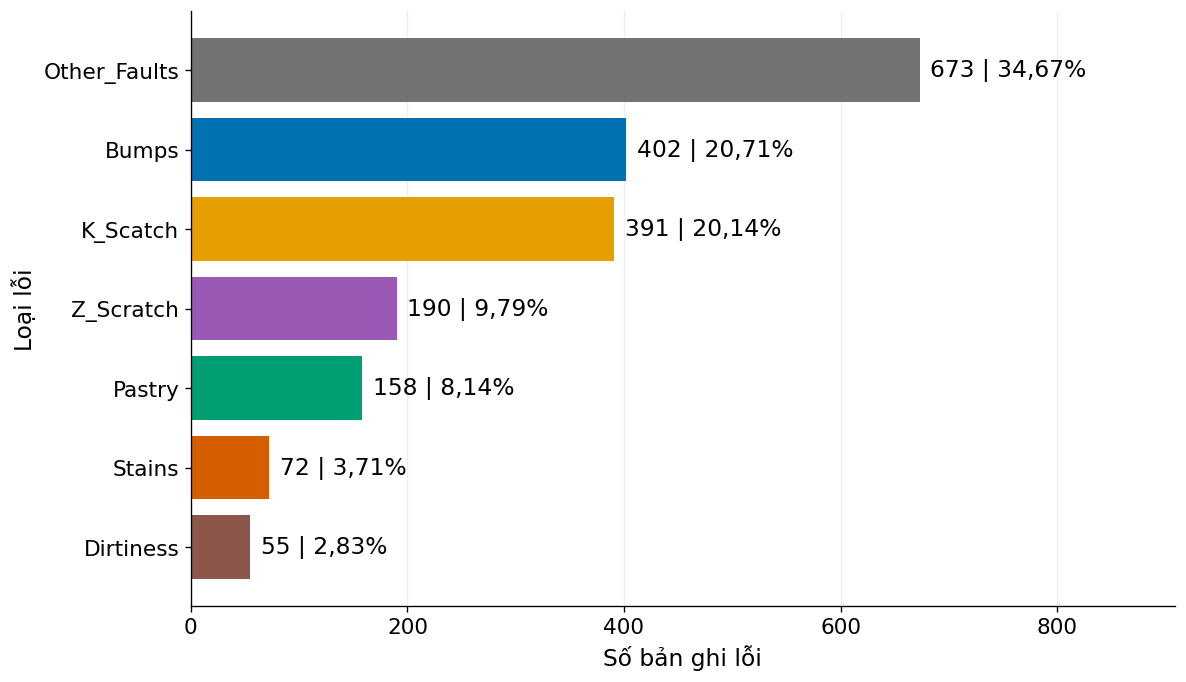
\includegraphics[width=\linewidth]{figures/chuong4/notebook_01_co_cau_loi.png}
\captionof{figure}{Other\_Faults đông nhất; Bumps và K\_Scatch chỉ chênh nhau 11 bản ghi}
\label{fig:ch4cocau}
\smallskip\par\footnotesize Nguồn: notebook bước 1--6, mục 5.2, Hình 1; 1.941 bản ghi sau làm sạch.
\end{minipage}\end{center}

\maCot{Other_Faults} đứng đầu với 673 bản ghi, chiếm 34,67\%. Tiếp theo là \maCot{Bumps} với 402 bản ghi (20,71\%) và \maCot{K_Scatch} với 391 bản ghi (20,14\%). Hai nhóm sau chỉ chênh nhau 11 bản ghi, tương đương khoảng 0,57 điểm phần trăm trên toàn tập. Ở cuối phân bố, \maCot{Dirtiness} có 55 bản ghi; cỡ mẫu lớn nhất gấp cỡ mẫu nhỏ nhất khoảng 12,24 lần.

Thứ hạng này cho thấy dữ liệu mất cân bằng giữa các nhãn. Nhóm đông sẽ tạo nhiều điểm hơn trên scatter, trong khi nhóm ít mẫu cần được đọc cùng cỡ mẫu khi so sánh phân bố. Riêng \maCot{Other_Faults} là nhãn gộp, chưa cho biết thành phần bên trong. Số lượng của nhóm vì vậy chưa xác định được một hiện tượng lỗi duy nhất để ưu tiên xử lý.

\begin{center}\begin{minipage}{\linewidth}
\centering
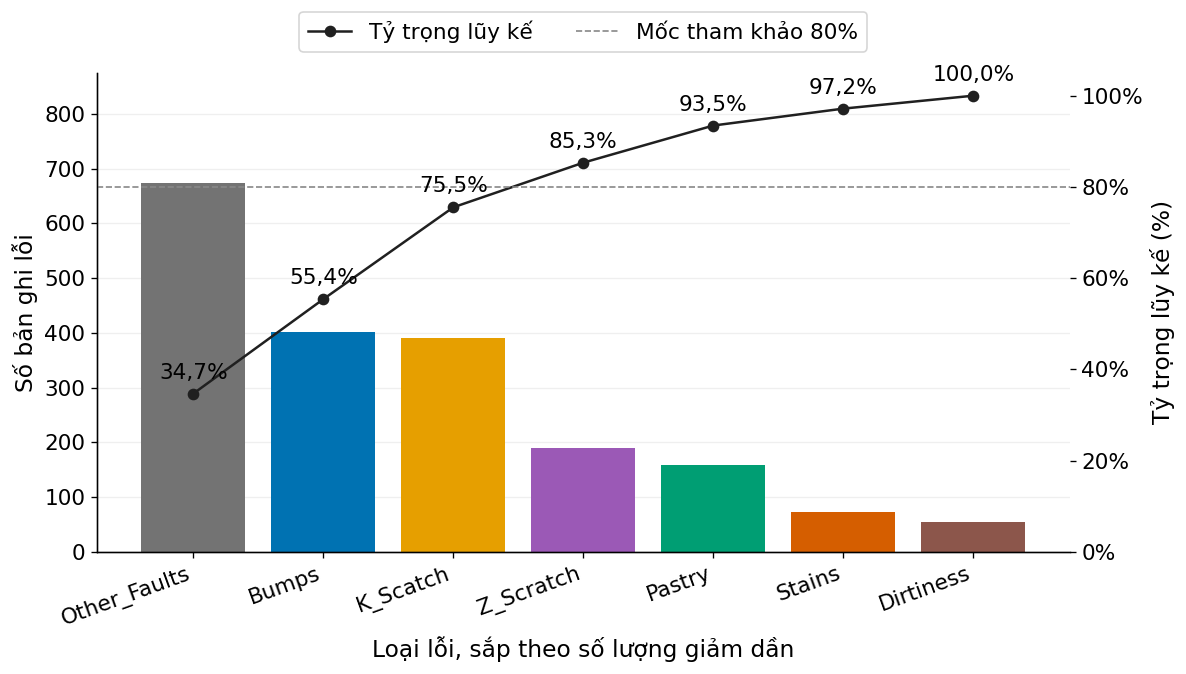
\includegraphics[width=\linewidth]{figures/chuong4/notebook_02_pareto_loi.png}
\captionof{figure}{Ba nhãn đầu chiếm 75,53\%; cần bốn nhãn để vượt mốc 80\%}
\label{fig:ch4pareto}
\smallskip\par\footnotesize Nguồn: notebook bước 1--6, mục 5.2, Hình 2; lũy kế theo số bản ghi lỗi.
\end{minipage}\end{center}

Đường lũy kế trong Hình~\ref{fig:ch4pareto} đặt mức tập trung đó vào toàn bộ cơ cấu. Ba nhãn đầu chứa 1.466 bản ghi, tương ứng 75,53\%; thêm \maCot{Z_Scratch} với 190 bản ghi thì lũy kế đạt 85,32\%. Mốc 80\% giúp đọc phạm vi bao phủ của các nhãn phổ biến, nhưng chưa có chi phí hay mức hạ cấp sản phẩm để chuyển thứ hạng này thành ưu tiên sản xuất. Để hiểu hai nhóm gần bằng nhau về tần suất, phần tiếp theo xét chúng nằm ở dòng thép nào.

\section{Q2: Bumps và K\_Scatch phân bố khác nhau theo dòng thép}
\label{sec:ch4q2}

Hình~\ref{fig:ch4thepsoluong} chia mỗi nhãn thành A300 và A400. Màu biểu diễn nhãn, họa tiết phân biệt dòng thép. Tổng cỡ mẫu là 777 bản ghi A300 và 1.164 bản ghi A400.

\begin{center}\begin{minipage}{\linewidth}
\centering
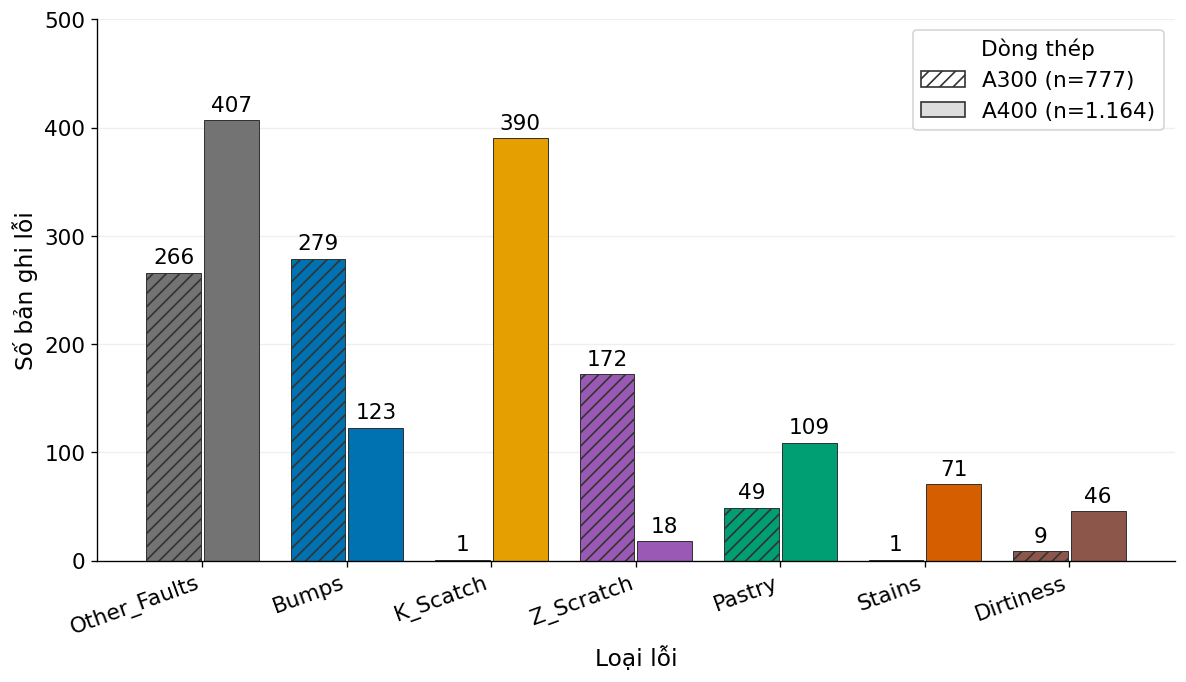
\includegraphics[width=\linewidth]{figures/chuong4/notebook_03_loi_theo_thep_so_luong.png}
\captionof{figure}{K\_Scatch gần như tập trung ở A400; Bumps có mặt đáng kể ở cả hai dòng thép}
\label{fig:ch4thepsoluong}
\smallskip\par\footnotesize Nguồn: notebook bước 1--6, mục 5.3, Hình 3; số đếm theo tổ hợp nhãn--dòng thép.
\end{minipage}\end{center}

\maCot{Bumps} gồm 279 bản ghi A300 và 123 bản ghi A400. Với \maCot{K_Scatch}, phân bố là một bản ghi A300 và 390 bản ghi A400. Dù số lượng toàn tập gần nhau, hai nhãn có vị trí rất khác trong bảng chéo. Ngoài \maCot{K_Scatch}, \maCot{Stains} tập trung ở A400 và \maCot{Z_Scratch} tập trung ở A300; cả ba vượt mốc mô tả 90\% trong từng nhãn theo công thức~\eqref{eq:tieuchiq2}.

\begin{center}\begin{minipage}{\linewidth}
\captionof{table}{Phân bố theo dòng thép cho thấy ba nhãn tập trung trên 90\%}
\label{tab:ch4taptrung}
\small\setstretch{1.1}
\begin{tabularx}{\linewidth}{@{}Y rrr r@{}}
\toprule
Nhãn & Tổng & A300 & A400 & \shortstack{Tỷ trọng ở dòng\\tập trung (\%)} \\
\midrule
\maCot{Other_Faults} & 673 & 266 & 407 & 60,48 (A400) \\
\maCot{Bumps} & 402 & 279 & 123 & 69,40 (A300) \\
\maCot{K_Scatch} & 391 & 1 & 390 & \textbf{99,74} (A400) \\
\maCot{Z_Scratch} & 190 & 172 & 18 & \textbf{90,53} (A300) \\
\maCot{Pastry} & 158 & 49 & 109 & 68,99 (A400) \\
\maCot{Stains} & 72 & 1 & 71 & \textbf{98,61} (A400) \\
\maCot{Dirtiness} & 55 & 9 & 46 & 83,64 (A400) \\
\bottomrule
\end{tabularx}
\smallskip\par\raggedright\footnotesize Mẫu số tỷ trọng là tổng bản ghi của từng nhãn; số liệu từ mục 5.3, bảng hỗ trợ Hình 3 trong notebook.
\end{minipage}\end{center}

Để so sánh cơ cấu khi hai dòng thép có cỡ mẫu khác nhau, Hình~\ref{fig:ch4theptytrong} đưa từng dòng về 100\%. Mẫu số lúc này chuyển sang tổng bản ghi lỗi của dòng thép đang xét.

\begin{center}\begin{minipage}{\linewidth}
\centering
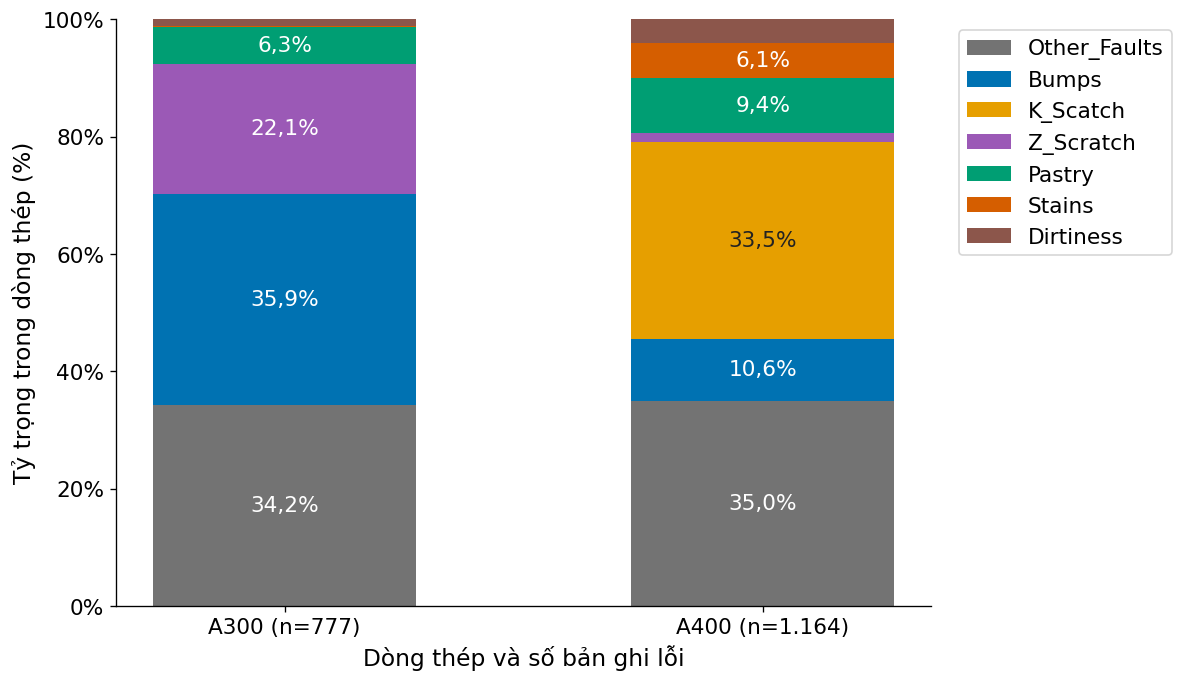
\includegraphics[width=\linewidth]{figures/chuong4/notebook_04_loi_theo_thep_ty_trong.png}
\captionof{figure}{Trong tập lỗi, A300 nổi bật Bumps và Z\_Scratch; A400 nổi bật K\_Scatch}
\label{fig:ch4theptytrong}
\smallskip\par\footnotesize Nguồn: notebook bước 1--6, mục 5.3, Hình 4; mỗi dòng thép cộng 100\%.
\end{minipage}\end{center}

Ở A300, \maCot{Bumps} chiếm 35,91\% và \maCot{Z_Scratch} chiếm 22,14\%. Ở A400, \maCot{K_Scatch} chiếm 33,51\%, còn \maCot{Bumps} chiếm 10,57\%. Tỷ trọng \maCot{Other_Faults} gần nhau, lần lượt 34,23\% và 34,97\%; khác biệt nổi bật nằm ở các nhãn cụ thể.

Với cùng 390 bản ghi \maCot{K_Scatch}/A400, phép chia $390/391$ cho 99,74\% mô tả dòng thép trong nhãn, còn $390/1.164$ cho 33,51\% mô tả nhãn trong dòng thép. Cả hai đều có mẫu số là bản ghi lỗi. Thiếu tổng sản lượng, chúng chưa cho biết xác suất phát sinh lỗi của A400. Sự tập trung quan sát được dẫn đến câu hỏi tiếp theo: đặc trưng độ sáng có giúp mô tả nhóm này cụ thể hơn không?

\section{Q3: Độ sáng tối thiểu làm rõ khác biệt ở phần trung tâm}
\label{sec:ch4q3}

Hình~\ref{fig:ch4scatter} đặt mỗi bản ghi tại cặp độ sáng tối thiểu--tối đa, giữ bảy màu nhãn và giảm độ đậm để thấy vùng chồng điểm. Các điểm \maCot{K_Scatch} màu cam tập trung nhiều về phía độ sáng tối thiểu thấp; nhiều nhãn khác cùng xuất hiện ở vùng trung tâm.

\begin{center}\begin{minipage}{\linewidth}
\centering
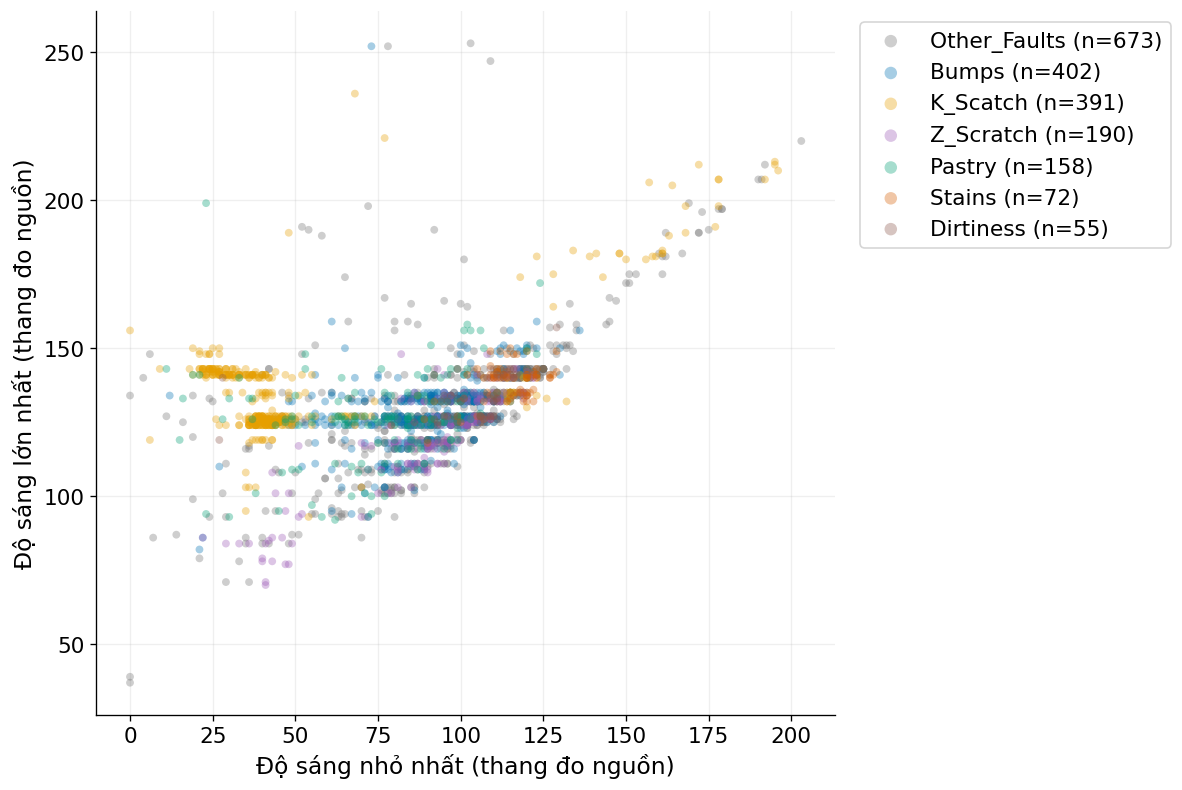
\includegraphics[width=\linewidth]{figures/chuong4/notebook_05_scatter_do_sang.png}
\captionof{figure}{K\_Scatch tập trung về phía độ sáng tối thiểu thấp, nhưng các điểm vẫn chồng lấn}
\label{fig:ch4scatter}
\smallskip\par\footnotesize Nguồn: notebook bước 1--6, mục 5.4, Hình 5; mỗi điểm là một bản ghi.
\end{minipage}\end{center}

Trung vị độ sáng tối thiểu của \maCot{K_Scatch} là 41, trong khi sáu nhãn còn lại có trung vị từ 80 đến 115. Khoảng P25--P75 của nhóm là 35--49; cận dưới nhỏ nhất của sáu khoảng còn lại là 64 ở \maCot{Pastry}. Bảng~\ref{tab:ch4dosang} giúp đọc chính xác phần trung tâm mà scatter khó thể hiện do điểm chồng nhau.

\begin{center}\begin{minipage}{\linewidth}
\captionof{table}{Phần trung tâm độ sáng tối thiểu của K\_Scatch khác biệt rõ hơn độ sáng tối đa}
\label{tab:ch4dosang}
\small\setstretch{1.1}
\begin{tabularx}{\linewidth}{@{}Y r p{2.3cm}r p{2.1cm}@{}}
\toprule
Nhãn & \shortstack{Trung vị\\Min} & P25--P75 Min & \shortstack{Trung vị\\Max} & P25--P75 Max \\
\midrule
\maCot{Other_Faults} & 97 & 80--111 & 127 & 119--140 \\
\maCot{Bumps} & 91 & 79,25--102 & 127 & 124--134 \\
\maCot{K_Scatch} & 41 & \textbf{35--49} & 134 & 126--141 \\
\maCot{Z_Scratch} & 93 & 81--104 & 124 & 111--132 \\
\maCot{Pastry} & 80 & 64--94 & 126 & 119--133 \\
\maCot{Stains} & 115 & 110--120 & 140 & 135--142 \\
\maCot{Dirtiness} & 107 & 96,5--111 & 132 & 127--140 \\
\bottomrule
\end{tabularx}
\smallskip\par\raggedright\footnotesize Min/Max: độ sáng tối thiểu/tối đa trên thang nguồn; thống kê từ mục 5.4, phần ``Tương quan và thống kê theo nhãn'' trong notebook.
\end{minipage}\end{center}

Khác biệt này chỉ áp dụng cho 50\% trung tâm. Toàn bộ độ sáng tối thiểu của \maCot{K_Scatch} trải từ 0 đến 196, vẫn chồng phạm vi của các nhóm khác; 297/391 bản ghi của nhãn có Min dưới 50 (75,96\%). Ở độ sáng tối đa, IQR 126--141 cũng chồng với nhiều nhãn. Vì vậy, dấu hiệu Min thấp là căn cứ lựa chọn đặc trưng để kiểm chứng, chưa tạo thành một ngưỡng gán nhãn.

Hệ số Pearson toàn tập là 0,4296, mô tả liên hệ tuyến tính dương giữa Min và Max. Giá trị này chưa đo khả năng phân loại lỗi. Tiêu chí không chồng IQR được bổ sung sau khi quan sát dữ liệu; cần đánh giá trên tập độc lập trước khi dùng cho nhận diện. Sau độ sáng, độ dày cung cấp thêm một chiều để xem sự tập trung của \maCot{K_Scatch} có đi cùng đặc điểm vật liệu hay không.

\section{Q4: Độ dày của K\_Scatch tập trung hẹp, thống kê gộp cần đọc cùng dòng thép}
\label{sec:ch4q4}

Hình~\ref{fig:ch4doday} là boxplot độ dày theo nhãn trên toàn tập, chưa tách A300/A400. \maCot{Other_Faults} có hộp rộng, trong khi hộp của \maCot{K_Scatch}, \maCot{Z_Scratch} và \maCot{Stains} co lại thành vạch vì P25 bằng P75.

\begin{center}\begin{minipage}{\linewidth}
\centering
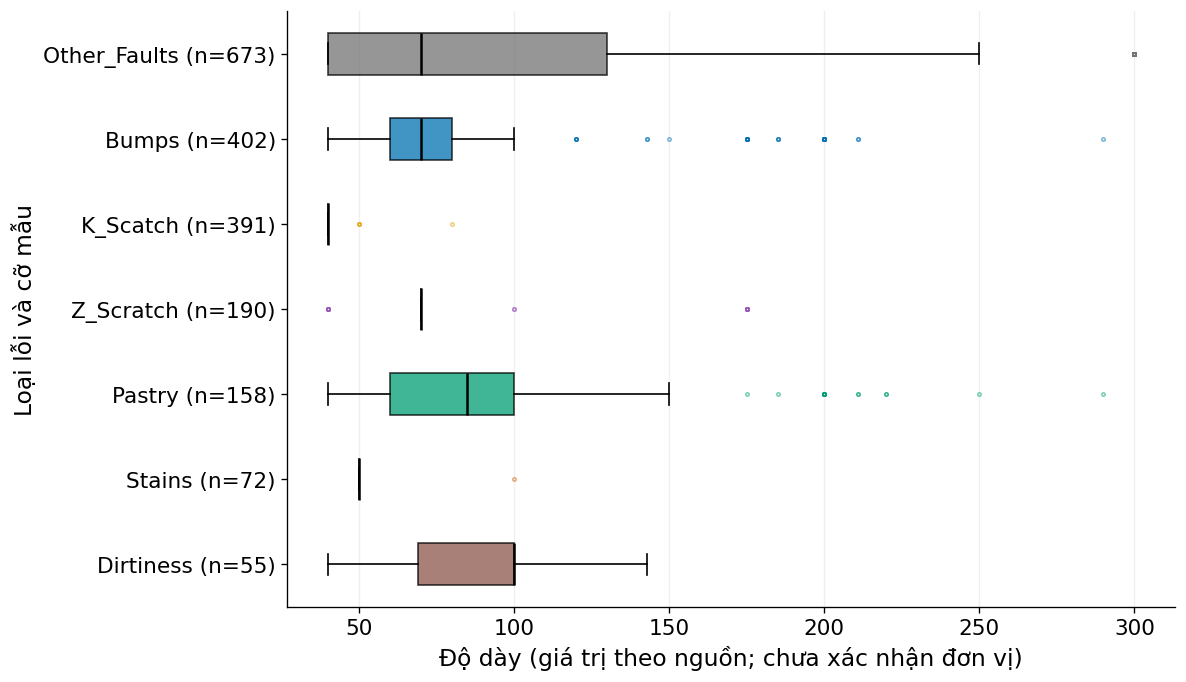
\includegraphics[width=\linewidth]{figures/chuong4/notebook_06_boxplot_do_day.png}
\captionof{figure}{K\_Scatch tập trung ở độ dày 40; Other\_Faults phân tán rộng hơn}
\label{fig:ch4doday}
\smallskip\par\footnotesize Nguồn: notebook bước 1--6, mục 5.5, Hình 6; độ dày theo thang nguồn, chưa xác nhận đơn vị.
\end{minipage}\end{center}

Toàn tập có trung vị độ dày 70 và 76,30\% bản ghi nằm trong khoảng 40--80. \maCot{K_Scatch} có trung vị 40, IQR bằng 0 và độ lệch chuẩn mẫu 2,20. Với \maCot{Other_Faults}, P25--P75 là 40--130; với \maCot{Bumps}, khoảng này là 60--80. IQR bằng 0 chưa đồng nghĩa với không biến thiên: \maCot{Z_Scratch} có IQR bằng 0 tại 70 nhưng độ lệch chuẩn mẫu vẫn là 24,70.

\begin{center}\begin{minipage}{\linewidth}
\captionof{table}{Trung vị gộp có thể che khác biệt độ dày giữa A300 và A400}
\label{tab:ch4doday}
\small\setstretch{1.1}
\setlength{\tabcolsep}{4pt}
\begin{tabularx}{\linewidth}{@{}Y r p{1.8cm}r p{2.2cm}p{2.2cm}@{}}
\toprule
Nhãn & \shortstack{Trung vị\\gộp} & P25--P75 & SD mẫu & \shortstack{A300\\Trung vị (N)} & \shortstack{A400\\Trung vị (N)} \\
\midrule
\maCot{Other_Faults} & 70 & 40--130 & 73,85 & 80 (266) & 50 (407) \\
\maCot{Bumps} & 70 & 60--80 & 38,05 & 70 (279) & 40 (123) \\
\maCot{K_Scatch} & 40 & 40--40 & 2,20 & 80 (1) & 40 (390) \\
\maCot{Z_Scratch} & 70 & 70--70 & 24,70 & 70 (172) & 175 (18) \\
\maCot{Pastry} & 85 & 60--100 & 51,59 & 80 (49) & 90 (109) \\
\maCot{Stains} & 50 & 50--50 & 5,89 & 100 (1) & 50 (71) \\
\maCot{Dirtiness} & 100 & 69--100 & 28,66 & 69 (9) & 100 (46) \\
\bottomrule
\end{tabularx}
\smallskip\par\raggedright\footnotesize Nguồn: mục 5.5 trong notebook, bảng hỗ trợ Hình 6 và ``Bảng bổ sung. Độ dày tách theo dòng thép''. N là cỡ mẫu; N=1 chỉ mô tả một bản ghi.
\end{minipage}\end{center}

Bảng bổ sung của notebook cho thấy \maCot{Bumps} có trung vị 70 ở A300 và 40 ở A400; \maCot{Other_Faults} có trung vị tương ứng 80 và 50. Đây là thông tin từ thống kê nhóm, bổ sung cho boxplot gộp. Hai tổ hợp \maCot{K_Scatch}/A300 và \maCot{Stains}/A300 chỉ có một quan sát; trung vị 175 của \maCot{Z_Scratch}/A400 cũng chỉ dựa trên 18 bản ghi.

Kết hợp Q2 và Q4 cho thấy dòng thép và độ dày đi cùng nhau rất chặt trong nhóm \maCot{K_Scatch}. Dữ liệu chưa đủ để tách ảnh hưởng riêng của từng yếu tố; thiếu sản lượng cũng chưa cho phép kết luận độ dày nào dễ phát sinh lỗi. Đặc điểm tiếp theo được xét là diện tích, nơi hai nhóm gần bằng nhau về số lượng có thể khác nhau nhiều về quy mô vùng lỗi.

\section{Q5: Diện tích làm rõ khác biệt và giải thích quyết định giữ các cờ IQR}
\label{sec:ch4q5}

Diện tích trải trên nhiều bậc độ lớn nên Hình~\ref{fig:ch4boxarea} dùng trục log cơ số 10. Boxplot vẫn được tính từ \maCot{Pixels_Areas} trên thang gốc, rồi mới đổi trục hiển thị. Khoảng cách bằng nhau trên trục thể hiện tỷ số bằng nhau; các điểm ngoài râu được giữ lại.

\begin{center}\begin{minipage}{\linewidth}
\centering
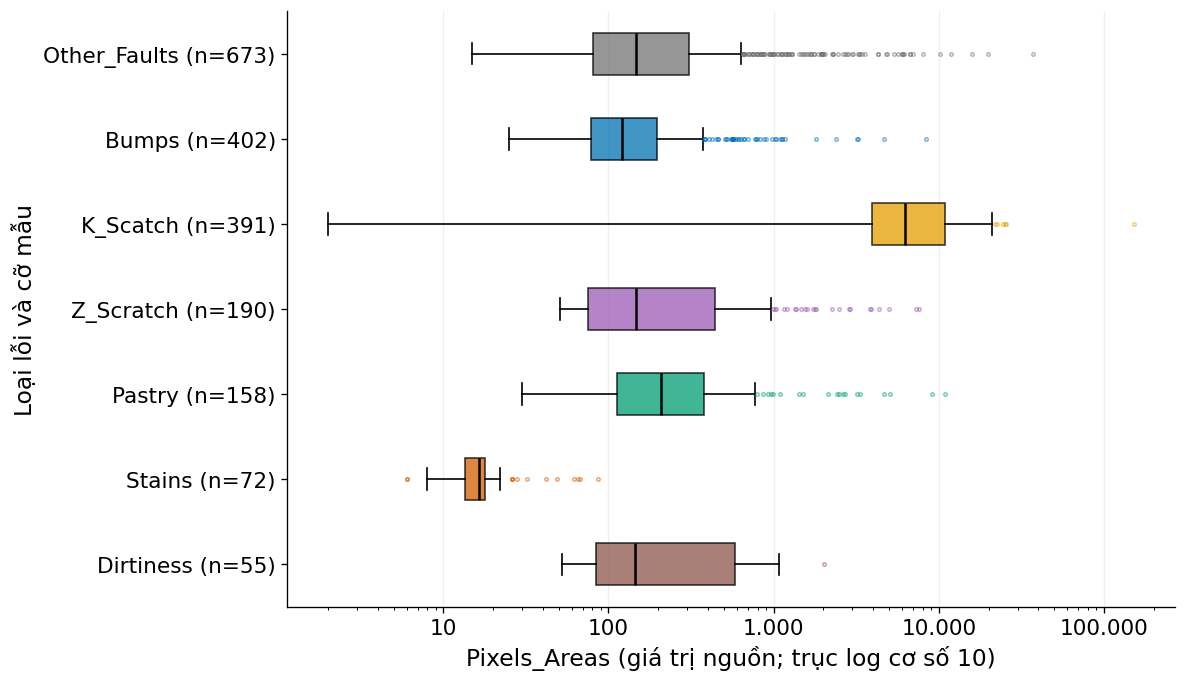
\includegraphics[width=\linewidth]{figures/chuong4/notebook_07_boxplot_dien_tich_log.png}
\captionof{figure}{K\_Scatch và Stains ở hai đầu của phân bố diện tích trung tâm}
\label{fig:ch4boxarea}
\smallskip\par\footnotesize Nguồn: notebook bước 1--6, mục 5.5, Hình 7; boxplot tính trên diện tích gốc, trục hiển thị log.
\end{minipage}\end{center}

Trung vị diện tích của \maCot{K_Scatch} là 6.281, lớn hơn khoảng 52,12 lần trung vị 120,5 của \maCot{Bumps}. \maCot{Stains} có trung vị nhỏ nhất, 16,5. IQR của \maCot{K_Scatch} là 3.948,5--10.908,5, nằm cao hơn IQR của các nhóm còn lại; \maCot{Stains} có IQR 13,5--18, nằm thấp hơn. Các nhãn ở giữa chồng nhau nhiều, nên diện tích đơn lẻ chưa mô tả đầy đủ khác biệt giữa chúng.

\begin{center}\begin{minipage}{\linewidth}
\captionof{table}{K\_Scatch có 326 cờ IQR toàn tập nhưng chỉ sáu điểm ngoài râu riêng của nhãn}
\label{tab:ch4area}
\small\setstretch{1.1}
\setlength{\tabcolsep}{4pt}
\begin{tabularx}{\linewidth}{@{}Y r p{3.0cm}rr@{}}
\toprule
Nhãn & Trung vị & P25--P75 & \shortstack{Ngoài râu\\từng nhãn} & \shortstack{Cờ IQR\\toàn tập} \\
\midrule
\maCot{Other_Faults} & 146 & 81--308 & 103 & 42 \\
\maCot{Bumps} & 120,5 & 78,25--197,5 & 44 & 5 \\
\maCot{K_Scatch} & 6.281 & 3.948,5--10.908,5 & \textbf{6} & \textbf{326} \\
\maCot{Z_Scratch} & 146 & 75,25--442 & 23 & 10 \\
\maCot{Pastry} & 209 & 112,5--381,25 & 19 & 11 \\
\maCot{Stains} & 16,5 & 13,5--18 & 13 & 0 \\
\maCot{Dirtiness} & 145 & 84,5--581,5 & 1 & 1 \\
\midrule
Tổng số bản ghi theo tiêu chí & & & 209 & 395 \\
\bottomrule
\end{tabularx}
\smallskip\par\raggedright\footnotesize Nguồn: mục 5.5, bảng hỗ trợ Hình 7 trong notebook. Điểm ngoài râu vượt hàng rào 1,5 × IQR tính riêng từng nhãn; cờ IQR toàn tập dùng một hàng rào chung cho 1.941 bản ghi.
\end{minipage}\end{center}

Phần trung tâm khác biệt chưa có nghĩa mọi quan sát đều tách nhau: diện tích \maCot{K_Scatch} trải từ 2 đến 152.655. Diện tích lớn cũng chưa đo được mức thiệt hại, vì dữ liệu thiếu tiêu chí chấp nhận và thông tin hạ cấp sản phẩm.

Hai cột cuối Bảng~\ref{tab:ch4area} trả lời vế giá trị ngoài râu của Q5: có 209 bản ghi nằm ngoài râu khi tính riêng từng nhãn, so với 395 cờ theo ngưỡng toàn tập. Riêng \maCot{K_Scatch}, 326/391 bản ghi bị gắn cờ toàn tập (83,38\%), nhưng chỉ 6/391 bản ghi nằm ngoài râu của chính nhãn (1,53\%). Chênh lệch này cho thấy nhiều bản ghi có diện tích lớn so với toàn tập vẫn nằm trong phạm vi râu của nhóm có diện tích trung tâm lớn.

Nếu loại tự động toàn bộ cờ, tập còn 1.546 dòng và \maCot{K_Scatch} còn 65 bản ghi, chỉ chiếm 4,20\%, thay vì 20,14\% ban đầu. Đây là phép đối chiếu giả định từ số cờ, không phải dữ liệu đã dùng để vẽ hình. Nó cho thấy ngưỡng chung có thể loại phần lớn một nhóm vốn có diện tích trung tâm lớn. Quyết định giữ các giá trị khớp nguồn ở Q0 vì vậy giúp bảo toàn đặc điểm đã quan sát.

\section{Đối chiếu kết quả trên dashboard và phạm vi kiểm thử}
\label{sec:ch4dashboard}

Dashboard cho phép chọn dòng thép, nhãn và khoảng độ dày rồi tính lại KPI, biểu đồ và bảng trên cùng tập con. Mục 6.3 ``Giao diện, bộ lọc và KPI'' của notebook kiểm tra bốn phạm vi ở Bảng~\ref{tab:ch4kpi}; mục 6.2, phần ``Đối chiếu cùng đầu vào với notebook bước 3--5'', đối chiếu bảng lỗi, cơ cấu, hai mẫu số tỷ trọng và thống kê đặc trưng với module dùng trong ứng dụng.

Hình~\ref{fig:ch4dashboard} ghi lại giao diện ứng dụng đang chạy khi chọn A400 và \maCot{K_Scatch}, giữ khoảng độ dày 40--300 của toàn nguồn. Bộ lọc và bốn KPI cùng xuất hiện trên màn hình, giúp đối chiếu phạm vi đang chọn với dòng tương ứng trong Bảng~\ref{tab:ch4kpi}.

\begin{center}\begin{minipage}{\linewidth}
\centering
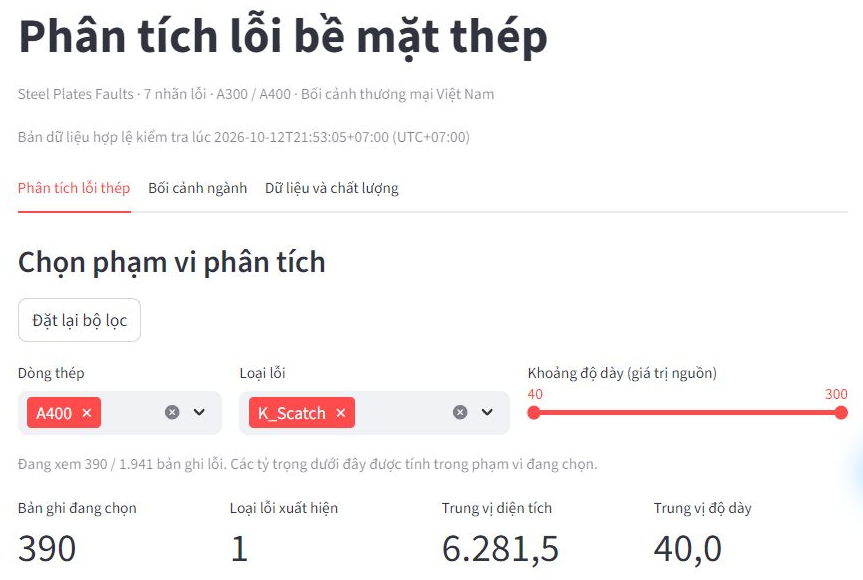
\includegraphics[width=\linewidth]{figures/chuong4/dashboard_a400_kscatch.png}
\captionof{figure}{Dashboard A400 và K\_Scatch: 390 bản ghi, một nhãn, trung vị diện tích 6.281,5 và độ dày 40,0}
\label{fig:ch4dashboard}
\smallskip\par\footnotesize Nguồn: ảnh chụp ứng dụng Streamlit đang chạy tại máy cục bộ ngày 12/10/2026; KPI được đối chiếu với mục 6.3 trong notebook.
\end{minipage}\end{center}

\begin{center}\begin{minipage}{\linewidth}
\captionof{table}{KPI theo phạm vi lọc nhất quán với các kết quả phân tích}
\label{tab:ch4kpi}
\small\setstretch{1.1}
\begin{tabularx}{\linewidth}{@{}Y rrrr@{}}
\toprule
Phạm vi & \shortstack{Số bản\\ghi} & \shortstack{Số\\nhãn} & \shortstack{Trung vị\\diện tích} & \shortstack{Trung vị\\độ dày} \\
\midrule
Toàn bộ & 1.941 & 7 & 174,0 & 70,0 \\
A300 & 777 & 7 & 113,0 & 70,0 \\
A400 và \maCot{K_Scatch} & 390 & 1 & 6.281,5 & 40,0 \\
Không chọn nhãn & 0 & 0 & -- & -- \\
\bottomrule
\end{tabularx}
\end{minipage}\end{center}

Khi thu hẹp vào A400 và \maCot{K_Scatch}, trung vị diện tích là 6.281,5 và trung vị độ dày là 40. Chênh lệch nhỏ với trung vị diện tích 6.281 ở Q5 đến từ việc bỏ bản ghi duy nhất của nhãn trên A300. Với tập rỗng, trung vị không xác định nên được để trống trong bảng tính và hiển thị dấu gạch trên giao diện.

Lần chạy lại bộ kiểm thử ngày 12/10/2026 lúc 21 giờ 53 phút (UTC+7) ghi nhận 11 ca đạt, không có lỗi, thất bại hay ca bỏ qua; kết quả được lưu tại \maCot{outputs/buoc_6/test_results.json} và đối chiếu trong mục 6.6 ``Kiểm tra ứng dụng'' của notebook. Các ca kiểm tra pipeline, bộ lọc, phạm vi rỗng, nạp nguồn và giữ bản hợp lệ, đồng thời xác nhận bốn KPI ở phạm vi A400 và \maCot{K_Scatch} khớp Bảng~\ref{tab:ch4kpi}. Lỗi API và chu kỳ cập nhật được mô phỏng; thử thay tệp thực hiện trên bản sao riêng. Kết quả này xác nhận hành vi trong các tình huống đã thử. Đánh giá với người dùng và theo dõi cập nhật dài hạn vẫn cần thực hiện thêm.

\section{Thảo luận và tiểu kết}
\label{sec:ch4thaoluan}

Qua bảy hình, \maCot{K_Scatch} chuyển từ nhãn phổ biến thứ ba thành một nhóm có các đặc điểm quan sát cụ thể: gần như tập trung ở A400, độ dày có trung vị 40 và phân tán hẹp, độ sáng tối thiểu thấp ở phần trung tâm, diện tích trung tâm lớn. \maCot{Bumps} có số lượng gần bằng nhưng trải trên cả hai dòng thép và diện tích nhỏ hơn nhiều. Những khác biệt này giúp chọn tổ hợp cần khảo sát; chúng chưa xếp hạng mức nghiêm trọng của lỗi.

\maCot{Stains} cũng có đặc điểm đáng chú ý: 71/72 bản ghi thuộc A400, trung vị độ dày 50 và trung vị diện tích 16,5. Với \maCot{Other_Faults}, số lượng lớn và phân bố rộng gợi ý cần làm rõ định nghĩa nhãn bằng ảnh bề mặt và thông tin QC trước khi phân chia nhóm. Các hướng này xuất phát từ mô tả trong mẫu, cần bằng chứng ngoài dữ liệu hiện tại để xác nhận.

Ba giới hạn chi phối cách sử dụng kết quả. Thứ nhất, thiếu tổng sản lượng và định danh tấm/cuộn khiến tỷ trọng bản ghi lỗi chưa trở thành tỷ lệ sản phẩm lỗi, đồng thời tính độc lập giữa các quan sát chưa được xác nhận. Thứ hai, thiếu biến vận hành và dữ liệu trong các tổ hợp dòng thép--độ dày nên chưa xác định nguyên nhân hoặc tách ảnh hưởng của từng yếu tố. Thứ ba, ngày là mô phỏng, đơn vị vật lý chưa được xác nhận đầy đủ và các tiêu chí khám phá được bổ sung sau khi xem dữ liệu.

Nguồn thương mại không có khóa liên hệ với các bản ghi lỗi, nên chỉ cung cấp bối cảnh độc lập, không giải thích những phân bố trong chương. Bước hoàn thiện tiếp theo là bổ sung sản lượng, định danh sản phẩm, thời gian thực, ảnh lỗi và mức thiệt hại; kiểm chứng dấu hiệu độ sáng trên tập độc lập; đồng thời đánh giá dashboard bằng nhiệm vụ sử dụng cụ thể. Việc giữ dữ liệu có căn cứ nguồn và ghi rõ mẫu số là cơ sở để các bước đó tiếp tục từ kết quả hiện tại.

Chương 4 đã nối kiểm tra dữ liệu với một câu chuyện phân tích từ cơ cấu nhãn đến đặc trưng từng nhóm. Hai nhãn \maCot{Bumps} và \maCot{K_Scatch} gần nhau về tần suất nhưng khác rõ ở dòng thép và diện tích trung tâm; độ sáng và độ dày bổ sung căn cứ mô tả. Đối chiếu 326 cờ toàn tập với sáu điểm ngoài râu riêng của \maCot{K_Scatch} làm rõ vì sao cần xem xét cấu trúc nhóm trước khi xử lý ngoại lai. Các kết quả xác lập những nội dung cần kiểm chứng tiếp và được chuyển thành phạm vi lọc có thể đối chiếu trên dashboard.

% ===== END: chuong/chuong4 =====
% ===== BEGIN: tailieu-thamkhao =====
\clearpage
\renewcommand{\bibname}{Tài liệu tham khảo}
\begin{thebibliography}{9}
  \addcontentsline{toc}{chapter}{Tài liệu tham khảo}

  \bibitem{uci}
  M. Buscema, S. Terzi và W. Tastle,
  \textit{Steel Plates Faults} [Bộ dữ liệu],
  UCI Machine Learning Repository, 2010.
  Giấy phép CC BY 4.0.
  \par\noindent
  DOI: \href{https://doi.org/10.24432/C5J88N}{10.24432/C5J88N}.
  Truy cập ngày 11/10/2026.

  \bibitem{reading}
  Đinh Nhật Anh, Nguyễn Thị Phương và Nguyễn Lê Ngọc Khôi,
  \textit{Phân tích nguy cơ xảy ra lỗi trong dây chuyền sản xuất thép},
  tài liệu đọc, không ghi năm, mục V.3.

  \bibitem{pandasmerge}
  pandas development team,
  \textit{pandas.merge}, tài liệu pandas.
  \par\noindent
  \url{https://pandas.pydata.org/docs/reference/api/pandas.merge.html}.
  Truy cập ngày 11/10/2026.

  \bibitem{nistbox}
  NIST/SEMATECH,
  \textit{e-Handbook of Statistical Methods},
  mục 1.3.3.7: Box Plot và mục 1.3.5.6: Measures of Scale.
  \par\noindent
  \url{https://www.itl.nist.gov/div898/handbook/eda/section3/boxplot.htm}.
  \par\noindent
  \url{https://www.itl.nist.gov/div898/handbook/eda/section3/eda356.htm}.
  Truy cập ngày 11/10/2026.

  \bibitem{niststats}
  National Institute of Standards and Technology (NIST),
  \textit{Dataplot Reference Manual}, mục Correlation.
  \par\noindent
  \url{https://www.itl.nist.gov/div898/software/dataplot/refman2/auxillar/correlat.htm}.
  Truy cập ngày 11/10/2026.

  \bibitem{matplotlib}
  Matplotlib development team,
  \textit{Quick start guide}, tài liệu Matplotlib.
  \par\noindent
  \url{https://matplotlib.org/stable/users/explain/quick_start.html}.
  Truy cập ngày 11/10/2026.

  \bibitem{streamlit}
  Streamlit,
  \textit{Widget behavior}, tài liệu Streamlit.
  \par\noindent
  \url{https://docs.streamlit.io/develop/concepts/architecture/widget-behavior}.\space
  Truy cập ngày 11/10/2026.

  \bibitem{kharal}
  A. Kharal,
  \textit{Explainable Artificial Intelligence Based Fault Diagnosis and Insight Harvesting for Steel Plates Manufacturing},
  arXiv:2008.04448, bản v1, 2020.
  \par\noindent
  \url{https://arxiv.org/abs/2008.04448}.
  Truy cập ngày 11/10/2026.
\end{thebibliography}

% ===== END: tailieu-thamkhao =====

\end{document}
